\documentclass[a4paper,12pt,twoside]{memoir}

% Castellano
\usepackage[spanish,es-tabla]{babel}
\selectlanguage{spanish}
\usepackage[utf8]{inputenc}
\usepackage[T1]{fontenc}
\usepackage{lmodern} % scalable font
\usepackage{microtype}
\usepackage{placeins}
\usepackage{lscape}
\usepackage{adjustbox}


\RequirePackage{booktabs}
\RequirePackage[table]{xcolor}
\RequirePackage{xtab}
\RequirePackage{multirow}

% Links
\PassOptionsToPackage{hyphens}{url}\usepackage[colorlinks]{hyperref}
\hypersetup{
	allcolors = {red}
}

% Ecuaciones
\usepackage{amsmath}

% Rutas de fichero / paquete
\newcommand{\ruta}[1]{{\sffamily #1}}

% Párrafos
\nonzeroparskip

% Huérfanas y viudas
\widowpenalty100000
\clubpenalty100000

% Evitar solapes en el header
\nouppercaseheads


\let\tmp\oddsidemargin
\let\oddsidemargin\evensidemargin
\let\evensidemargin\tmp
\reversemarginpar



% Imagenes
\usepackage{graphicx}
\newcommand{\imagen}[2]{
	\begin{figure}[!h]
		\centering
		\includegraphics[width=0.9\textwidth]{#1}
		\caption{#2}\label{fig:#1}
	\end{figure}
	\FloatBarrier
}






\graphicspath{ {./img/} }

% Capítulos
\chapterstyle{bianchi}
\newcommand{\capitulo}[2]{
	\setcounter{chapter}{#1}
	\setcounter{section}{0}
	\setcounter{figure}{0}
	\setcounter{table}{0}
	\chapter*{#2}
	\addcontentsline{toc}{chapter}{#2}
	\markboth{#2}{#2}
}

% Apéndices
\renewcommand{\appendixname}{Apéndice}
\renewcommand*\cftappendixname{\appendixname}

\newcommand{\apendice}[1]{
	%\renewcommand{\thechapter}{A}
	\chapter{#1}
}

\renewcommand*\cftappendixname{\appendixname\ }

% Formato de portada
\makeatletter
\usepackage{xcolor}
\newcommand{\tutor}[1]{\def\@tutor{#1}}
\newcommand{\tutorb}[1]{\def\@tutorb{#1}}
\newcommand{\course}[1]{\def\@course{#1}}
\definecolor{cpardoBox}{HTML}{E6E6FF}
\def\maketitle{
  \null
  \thispagestyle{empty}
  % Cabecera ----------------
\begin{center}
  \noindent
\includegraphics[width=\textwidth]{cabeceraSalud}\vspace{1.5cm}%
\end{center}
  
  % Título proyecto y escudo salud ----------------
  \begin{center}
    \begin{minipage}[c][1.5cm][c]{.20\textwidth}
        
\includegraphics[width=\textwidth]{escudoSalud.pdf}
    \end{minipage}
  \end{center}
  
  \begin{center}
    \colorbox{cpardoBox}{%
        \begin{minipage}{.8\textwidth}
          \vspace{.5cm}\Large
          \begin{center}
          \textbf{TFG del Grado en Ingeniería de la Salud}\vspace{.6cm}\\
          \textbf{\LARGE\@title{}}
          \end{center}
          \vspace{.2cm}
        \end{minipage}
    }%
  \end{center}
  
    % Datos de alumno, curso y tutores ------------------
  \begin{center}%
  {%
    \noindent\LARGE
    Presentado por \@author{}\\ 
    en Universidad de Burgos\\
    \vspace{0.5cm}
    \noindent\Large
    \@date{}\\
    \vspace{0.5cm}
    %Tutor: \@tutor{}\\ % comenta el que no corresponda
    Tutores: \@tutor{} -- \@tutorb{}\\
  }%
  \end{center}%
  \null
  \cleardoublepage
  }
\makeatother



% Datos de portada
\title{título del TFG \\Documentación Técnica}
\author{nombre alumno}
\tutor{nombre tutor}
\tutorb{nombre tutor 2}
\date{\today}

\begin{document}

\maketitle



\cleardoublepage



%%%%%%%%%%%%%%%%%%%%%%%%%%%%%%%%%%%%%%%%%%%%%%%%%%%%%%%%%%%%%%%%%%%%%%%%%%%%%%%%%%%%%%%%



\frontmatter


\clearpage

% Indices
\tableofcontents

\clearpage

\listoffigures

\clearpage

\listoftables

\clearpage

\mainmatter

\appendix




\apendice{Plan de Proyecto Software}

\section{Introducción}

La intención de este anexo es la de dar a entender el plan de proyecto que se ha seguido a la hora de realizar este trabajo.

Primero se hablará sobre la planificación temporal seguida y más adelante su viabilidad tanto económica cómo legal

Las metodologías ágiles (especialmente Scrum) utilizadas en el desarrollo de este proyecto son aquellas que permiten ir adaptando la forma y carga de trabajo a medida que se desarrolla el proyecto, analizando los nuevos retos que pueden surgir durante la realización del mismo lo que otorga flexibilidad al proyecto durante la etapa de desarrollo.\cite{gomez_aplicacion_2020}

\subsection{Scrum}

Scrum es un marco ligero que ayuda a las personas, equipos y organizaciones a generar valor a través de soluciones adaptables para problemas complejos.

En la figura \ref{fig:scrum} se puede ver una ilustración del proceso de Scrum

Está basado en el empirismo y emplea un enfoque iterativo e incremental para el desarrollo del producto minimizando riesgos ya que en el caso de un desastre simplemente habría que dar marcha atrás hasta la última versión estable.

Esta metodología tiene dos pilares clave, El equipo Scrum y los eventos.

\begin{figure}[!h]
    \centering
    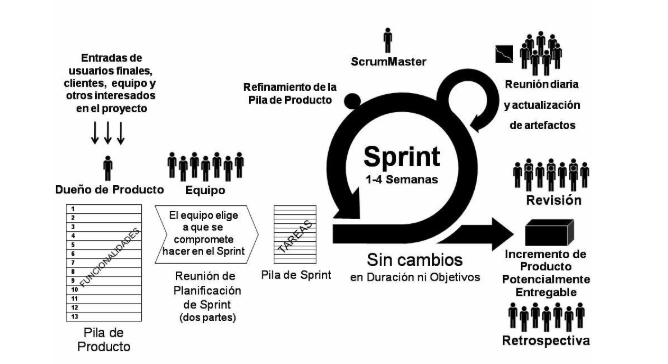
\includegraphics[width=1\textwidth]{img/Scrum.png}
    \caption{Ilustración del proceso de Scrum}
    \label{fig:scrum}
\end{figure}

\subsection{Equipo Scrum}

El capital humano que se encarga de desarrollar el proyecto. Constan de desarrolladores, product owner, Scrum Master.

\subsubsection{Desarrolladores}

Son los encargados de crear cada incremento al producto cada sprint.

Sus tareas dentro del ciclo Scrum son la de crear un plan para el sprint llamado Sprint Backlog, Adaptar su plan de desarrollo día a día según los objetivos del sprint y responsabilizarse del trabajo de sus compañeros desarrolladores para garantizar un buen trabajo de todas las partes.

\subsubsection{product owner}

El propietario del producto, es el responsable de sacar el máximo valor al trabajo del equipo Scrum así cómo gestionar la Backlog comunicando los objetivos a los que se desea llegar, se asegura de que se alcanza una buena calidad del producto final y gestionando los proyectos pendientes a realizar en el sprint.

\subsubsection{Scrum Master}

El máximo responsable de cumplir con la guía de Scrum, explicando cuidadosamente su teoría al resto del equipo así cómo coordinando su puesta en práctica.

Se responsabiliza de la efectividad del equipo Scrum eliminando las barreras entre los miembros, formándolos en la metodología y ayudándolos en sus planificaciones y tareas.


\subsection{Eventos de Scrum}

Los eventos en Scrum son oportunidades señaladas en el tiempo para revisar y adaptar los artefactos de Scrum, se crean para crear una regularidad y minimizar reuniones imprevistas.

\subsubsection{El Sprint}

Eventos de longitud fija donde ocurre todo el trabajo y en el que se fijan distintos objetivos.

En estos sprints iterativos se buscan realizar cambios que no deterioren el objetivo del sprint ni disminuya su calidad y clarificar los objetivos revaluando las tareas pendientes a medida que se desarrolla el proyecto.

\subsubsection{Planificación de Sprint}

Este evento inicia el Sprint estableciendo los objetivos a realizar en el mismo, este evento requiere de la participación del equipo de Scrum al completo.

Se pretende responder las siguientes cuestiones:

\begin{itemize}

    \item ¿Por qué este Sprint es valioso?
    \item ¿Qué se puede hacer este Sprint?
    \item ¿Cómo se realizará el trabajo elegido?

\end{itemize}

\subsubsection{Scrum diario}

Su propósito es el análisis del avance hacia el objetivo final del Sprint.
Es un evento de corta duración para los desarrolladores en los que discuten las diversas tareas del día.

\subsubsection{Revisión del Sprint}

Este evento que sucede al finalizar un Sprint tiene cómo propósito analizar este mismo, se revisan los logros conseguidos, los cambios que han tenido lugar y objetivos futuros.

\subsubsection{La retrospectiva del Sprint}

El objetivo de este último evento es el de aumentar la calidad del proyecto analizando el anterior sprint determinando que fue bien en el mismo, así cómo dificultades y la resolución o no de éstas.

Este evento concluye el Sprint

\subsection{Artefactos de Scrum}

Son la representación de los objetivos tanto a corto como a largo plazo del proyecto.

\subsubsection{Pila del producto}

Es una lista ordenada de lo que se necesita para mejorar el producto, los ítems en la pila del producto se consideran listos para su selección en un evento de planificación de Sprint.

\subsubsection{Pila del Sprint}

El trabajo pendiente por hacer en el Sprint. Se puede entender como el trabajo que aún le queda a los desarrolladores para alcanzar el objetivo de ese sprint.

\subsubsection{Incremento}

El incremento es cada pequeño objetivo cumplido que aporta un paso más hacia completar el objetivo del Sprint. Cada incremento es aditivo y deben funcionar todos juntos para llegar a la meta final. \cite{} Citar manual de Scrum %TODO

\footnote{Los anexos deben de tener su propia bibliografía, eso es tan fácil como utilizar referencias igual que en la memoria \cite{bortolot2005}}

\section{Planificación temporal}

Para la realización de este trabajo se ha seguido la metodología Scrum mediante la aplicación de Zube.io lo que ha dado lugar a la Siguiente planificación mediante Sprints.

\subsubsection{Sprint 1: Sprint inicial}

En este primer Sprint se pretendía tener una toma de contacto inicial con las herramientas que se iban a desarrollar a lo largo del proyecto, en especial se asignaron dos objetivos principales, familiarizarse con el entorno de Zube así como investigar las tecnologías de RAG y de LLMs.

\ref{fig:sprintinicial}

\subsubsection{Sprint 2: Prueba de modelos}

Segundo Sprint del proyecto, el objetivo era investigar los diferentes modelos de LLM, sus respuestas ante datos clínicos y cómo implementarlos, así cómo sus formas de pago si lo requiriese.

\ref{fig:pruebamodelos}

\subsubsection{Sprint 3: Creación del primer modelo funcional}

En este Sprint se creó el primer chatbot funcional con la primera implementación del proceso de RAG con los datos finales sacados de PubMed. También se empezó con el desarrollo de la memoria.

\ref{fig:modelofuncional}

\subsubsection{Sprint 4: Mejoras}

En este pequeño Sprint se creó el repositorio en GitHub y se realizaron mejoras al código del modelo, eliminando código innecesario.

\ref{fig:mejoras}

\subsubsection{Sprint 5: Marco Teórico}

Este Sprint tenía cómo objetivo inicial la creación de una interfaz gráfica web en streamlit, lamentablemente aparecieron multitud de problemas con la GPU permitida y se decidió dejarla en la backlog list. Al final en este sprint se realizó el desarrollo del marco teórico de la memoria.

\ref{fig:teorico}

\subsubsection{Sprint 6: Finalización del Marco Teórico y actualización de Anexos}

En este Sprint se finaliza lo empezado en el anterior sprint y se empieza a trabajar en los anexos, sobre todo en el de Planificación y Datos así cómo se investigó el anexo de sostenibilidad.

\ref{fig:anexos}

\subsubsection{Sprint 7: Creación de la interfaz gráfica de usuario, validación del modelo y trabajo en los anexos}

El objetivo principal de este sprint fue el de acabar la herramienta añadiendo la interfaz gráfica de usuario, es decir la parte visual que comunicará al usuario con el software del programa para hacerlo más manejable gestionando las entradas y mostrando las salidas, además se empezó a trabajar en la validación del modelo, creando una escala numérica en la que el desarrollador, otros LLMs y personas ajenas al proyecto que cumplen el rol de futuros usuarios, dieron su opinión interactuando con el modelo y puntuandolo en dicha escala numérica. Mientras este trabajo se desarrollaba también se actualizaban los anexos de la documentación del proyecto.

\subsubsection{Sprint board}

\begin{figure}[h!]
    \centering
    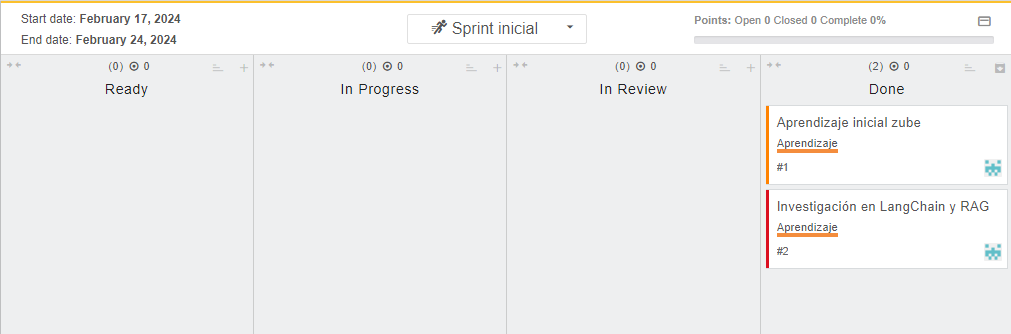
\includegraphics[width=1\textwidth]{img/SprintInicial.png}
    \caption{Sprint Inicial}
    \label{fig:sprintinicial}
\end{figure}

\begin{figure}[h!]
    \centering
    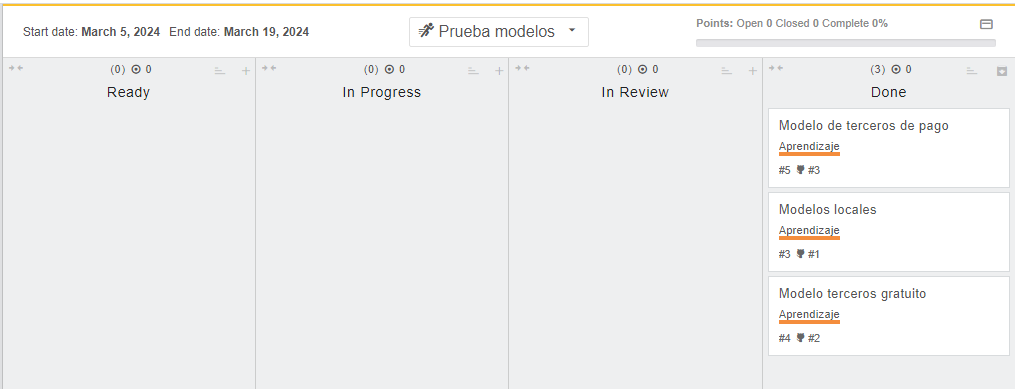
\includegraphics[width=1\textwidth]{img/PruebaModelos.png}
    \caption{Sprint Prueba Modelos}
    \label{fig:pruebamodelos}
\end{figure}

\begin{figure}[h!]
    \centering
    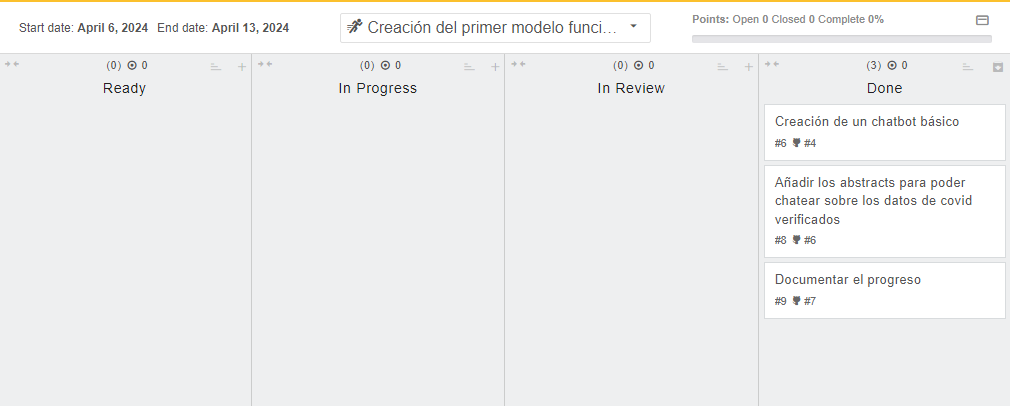
\includegraphics[width=1\textwidth]{img/modelofuncional.png}
    \caption{Sprint creación del primer modelo funcional}
    \label{fig:modelofuncional}
\end{figure}

\begin{figure}[h!]
    \centering
    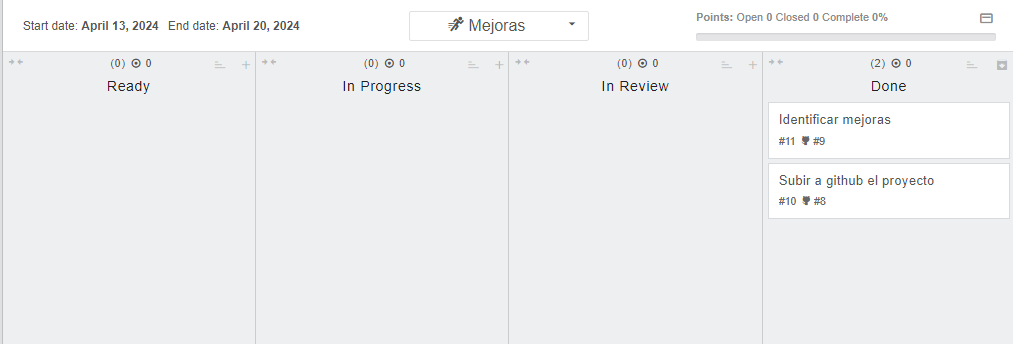
\includegraphics[width=1\textwidth]{img/Mejoras.png}
    \caption{Sprint Mejoras}
    \label{fig:mejoras}
\end{figure}

\begin{figure}[h!]
    \centering
    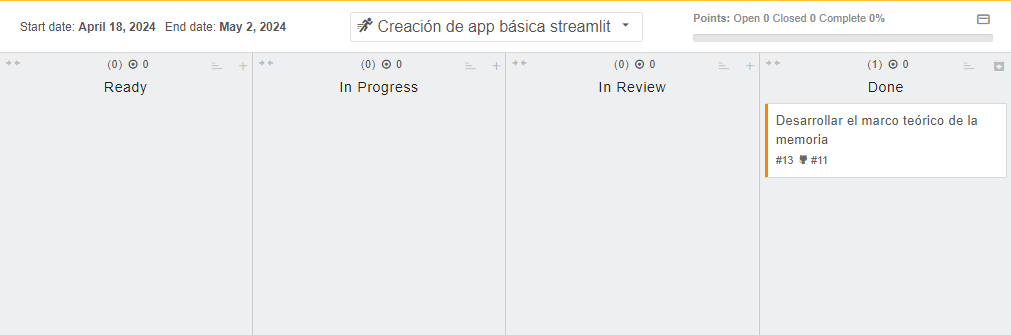
\includegraphics[width=1\textwidth]{img/teorico.png}
    \caption{Sprint Marco Teórico}
    \label{fig:teorico}
\end{figure}

\begin{figure}[h!]
    \centering
    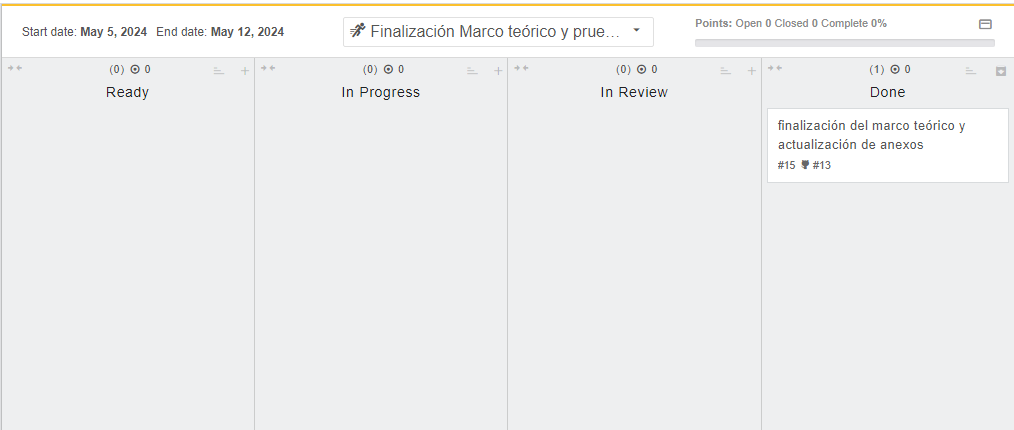
\includegraphics[width=1\textwidth]{img/anexos.png}
    \caption{Sprint Anexos}
    \label{fig:anexos}
\end{figure}

\begin{figure}[h!]
    \centering
    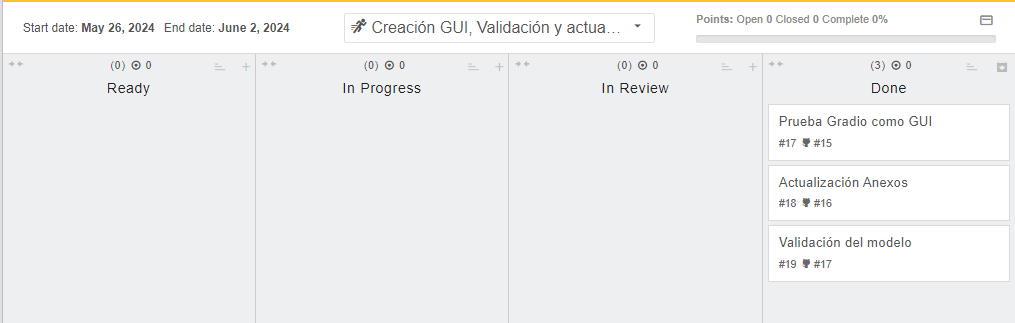
\includegraphics[width=1\textwidth]{img/gui.png}
    \caption{Sprint GUI}
    \label{fig:gui}
\end{figure}

\FloatBarrier

%TODO ir acabando los sprints a medida que los acabe

\subsection{Planificación económica}

En este apartado se analizarán los costes monetarios de la implementación del proyecto

\subsubsection{Librerías}
%TODO De momento todo lo empleado es de código abierto pero podría cambiar

Las librerías empleadas en el desarrollo han sido de código abierto por lo que no suman ningún coste.

\subsubsection{Contratación}

Se estima que el sueldo promedio de un programador Junior en España sería de 1750 euros brutos al mes a la fecha de realización de este proyecto como indica en la figura \ref{fig:Salario}, asumiendo que los pluses y complementos así cómo la parte proporcional de las pagas extra está incluida. \cite{} %TODO Inserar cita a la página web

\begin{figure}[h!]
    \centering
    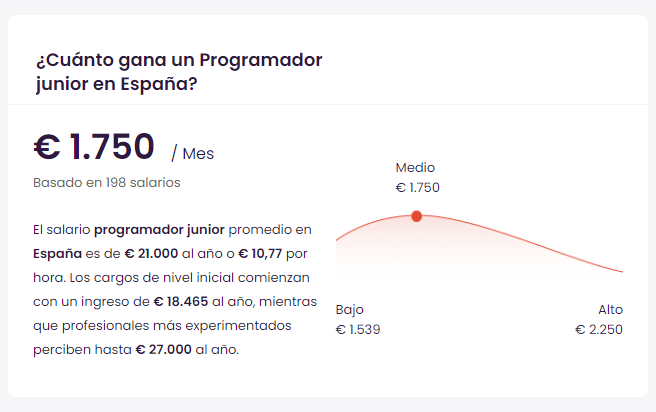
\includegraphics[width=1\textwidth]{img/Salario.png}
    \caption{Salario de un Programador Junior en España}
    \label{fig:Salario}
\end{figure}

También asumimos de manera arbitraria ya que esto cambiará dependiendo de multitud de condiciones un 9\% de Retención de IRPF y unas cotizaciones, enfermedad profesional y accidentes de trabajo del 35\%.

El resultado del cálculo sería una base de cotización de 1750 euros a los que se le tendrán que sumar los costes de la seguridad social que ascienden hasta los 1246.88 euros calculados teniendo en cuenta lo siguiente:

\begin{itemize}

    \item 23.60\% contingencias comunes
    \item 5.5\% tipo general de desempleo para un contrato indefinido
    \item 0,20\% FOGASA (Fondo de Garantía Salarial)
    \item 0,70\% formación profesional

\end{itemize}

A esa cantidad hay que sustraer el coste del empleado que será de 111.13 euros por lo que el coste que asumirá la empresa será de 1246.88 - 111.13 = 1135.75 que si sumamos al sueldo original el coste de contratar a un programador junior al mes asciende a los 1750 + 1135.75 = 2885.75 euros al mes 
%TODO insertar cita calculadora de coste de contratación

\subsubsection{Web}

Si se quisiera desplegar la aplicación Gradio ofrece hosting a través de los spaces de Hugging Face que puede ser gratuito o de pago. Teniendo en cuenta la GPU necesaria para ejecutar los modelos, sería conveniente emplear las opciones de pago que facilitan la aceleración de GPU, Hugging Face ofrece el espacio NVidia T4 small * 4vCPU * 15GB por 0,40 Dólares la hora, declarándose "dormidos" tras una hora de inactividad, este tiempo no se cobra.
%TODO insertar cita de los espacios de Huggin Face

\subsection{Viabilidad legal}
\subsubsection{Licencias}
Las librerías empleadas son Open Source.

Las licencias de las librerías empleadas son las siguientes:

\begin{itemize}

    \item Licencia de Python Software Foundation
    \item Licencia BSD modificada
    \item Licencia Apache 2.0
    \item Licencia MIT

\end{itemize}

\subsubsection{Legislación}

Según la Ley de inteligencia artificial publicada el 13 de marzo de 2024 las inteligencias artificiales se pueden clasificar en cuatro grupos según su riesgo:

\begin{itemize}

    \item Riesgo inaceptable
    \item Riesgo alto
    \item Riesgo limitado
    \item Riesgo mínimo o nulo

\end{itemize}

Cuando una inteligencia artificial presente una clara amenaza para la seguridad y/o los derechos de las personas estas estarán catalogadas cómo de riesgo inaceptable y, por lo tanto, prohibidas.

Las IAs que se empleen en infraestructuras críticas, formación profesional, componentes de seguridad, gestión de empleo, servicios públicos y privados esenciales, administración de justicia o gestión de la migración serán considerados de alto riesgo.

Estas IAs estarán sujetas a estrictas regulaciones cómo, exhaustivos controles de calidad, registros de actividad constantes y medidas adecuadas de supervisión humana.

Los riesgos limitados incluyen a los que puedan presentar problemas relacionados a la falta de transparencia en el uso de las mismas. Por ello sólo se permitirán aquellas IAs de Riesgo limitado las cuales aporten la suficiente información a su usuario.
Un ejemplo de esto sería un chatbot que sólo estaría permitido en el caso de que no hubiese ninguna en la interacción hombre-máquina, es decir, que el usuario siempre sea consciente que no está chateando con una persona real.

Las IAs de riesgo nulo cómo los filtros de spam o las usadas en videojuegos no tienen restricciones.

El proyecto cumple con la Ley de inteligencia artificial ya que se trata de una inteligencia artificial de Riesgo limitado en la que los usuarios en todo momento conocen que están interactuando con una máquina. %TOD insertar cita sobre la ley europea de IA

\apendice{Documentación de usuario}

\section{Requisitos software y hardware para ejecutar el proyecto.}

\subsection{Requisitos software}

Las librerías necesarias para este proyecto se encuentran al principio del proyecto para su instalación en servicios en linea con aceleración de GPU pero en el caso de su instalación en local se encontrarán en el archivo requirements.txt, también para ejecutarlo en local se deberá tener Python y pp instalado %TODO Crear el archivo requirements.

\subsection{Requisitos hardware}

No se recomienda la ejecución en local del programa, sin embargo se ha realizado una medición de la gpu necesaria para ejecutar el proyecto ya que es el aspecto más exigente, se puede ver en la figura \ref{fig:hardware}.

%TODO cambiar la imagen de abajo

\begin{figure}[h!]
    \centering
    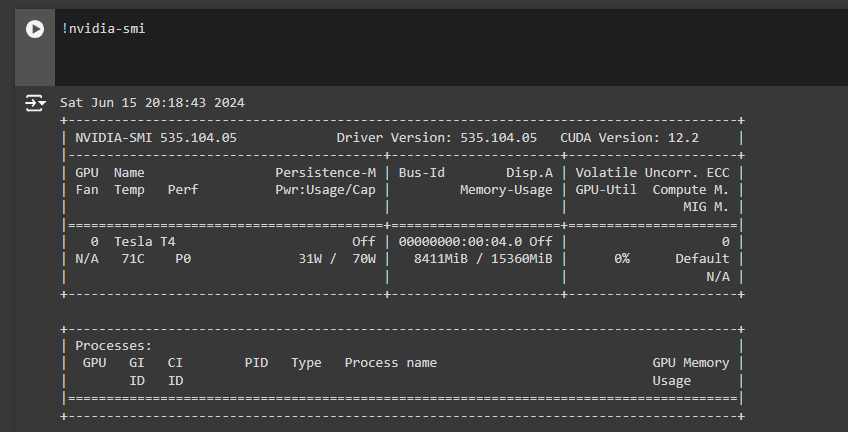
\includegraphics[width=1\textwidth]{img/hardware.png}
    \caption{Requisitos de GPU}
    \label{fig:hardware}
\end{figure}

\section{Instalación / Puesta en marcha}

Debido a que no se creó un espacio en Hugging Face que pueda soportar de forma permanente los grandes requisitos de GPU del proyecto se recurre a demos temporales.

Para visualizar la prueba de concepto simplemente hay que ejecutar el código presente en el repositorio en un entorno con suficiente GPU, por ejemplo, Kaggle o Google colab y acceder al link que se creará al final de la ejecución.

Para su puesta en marcha en local se deberá clonar el repositorio en github e instalar en el entorno deseado el archivo requirements.txt con el siguiente comando pip install -r requirements.txt siempre y cuando se tenga instalado tanto Python como pip en el sistema.


\section{Manuales y/o Demostraciones prácticas}

En este ejemplo se ejecutará el proyecto desde google colab empleando la aceleración por hardware T4 la cual será suficiente para la ejecución del proyecto, esto se podrá seleccionar desde la opción en el panel superior Entorno de ejecución -> Cambiar tipo de entorno de ejecución  y seleccionar un acelerador por hardware suficiente para ejecutar el proyecto, T4 es suficiente como se ve en la figura \ref{fig:aceleracion}.


\begin{figure}[h!]
    \centering
    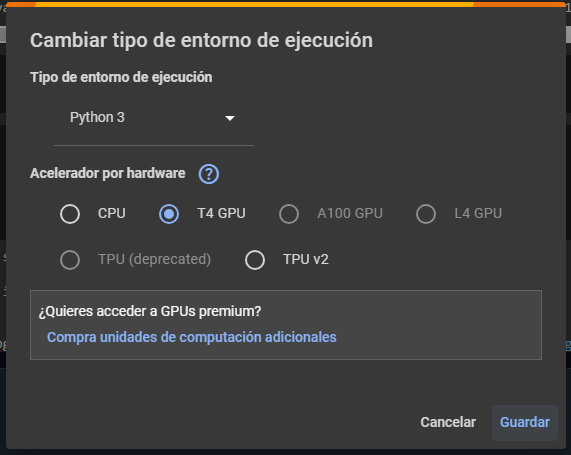
\includegraphics[width=1\textwidth]{img/aceleracion.png}
    \caption{Demostración de aceleración por hardware}
    \label{fig:aceleracion}
\end{figure}


Una vez ejecutado el proyecto se abrirá al final una ventana con la que se podrá interactuar con el modelo y un link con el que se podrá interactuar con el en línea y compartirlo para que se pueda acceder a él desde distintos dispositivos, el ejemplo de la interfaz vacía se puede ver en la figura \ref{fig:guivacia}.

\begin{figure}[h!]
    \centering
    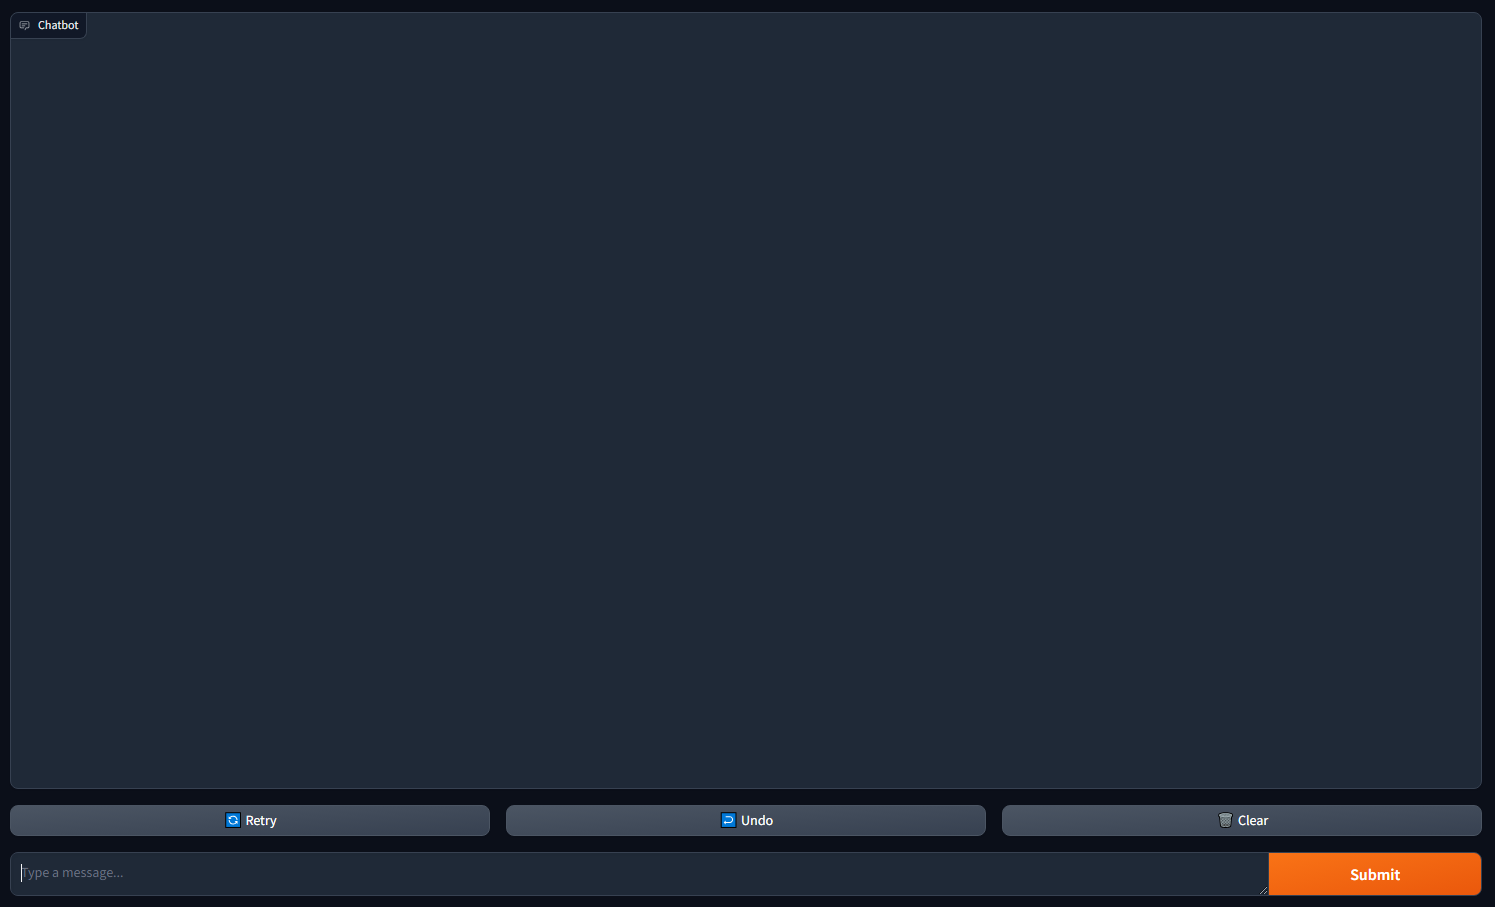
\includegraphics[width=1\textwidth]{img/guivacia.png}
    \caption{Interfaz gráfica de usuario}
    \label{fig:guivacia}
\end{figure}

Una vez ejecutada simplemente falta insertar el prompt deseado y seleccionar submit, luego, el modelo arrojará una respuesta con los abstracts que haya interpretado como los más relevantes según el prompt del usuario y la respuesta del prompt enriquecido con dichos abstracts obteniendo así la salida esperada de la respuesta al prompt inicial y bibliografía que la apoye, se puede ver en la figura \ref{fig:guirellena}

\begin{figure}[h!]
    \centering
    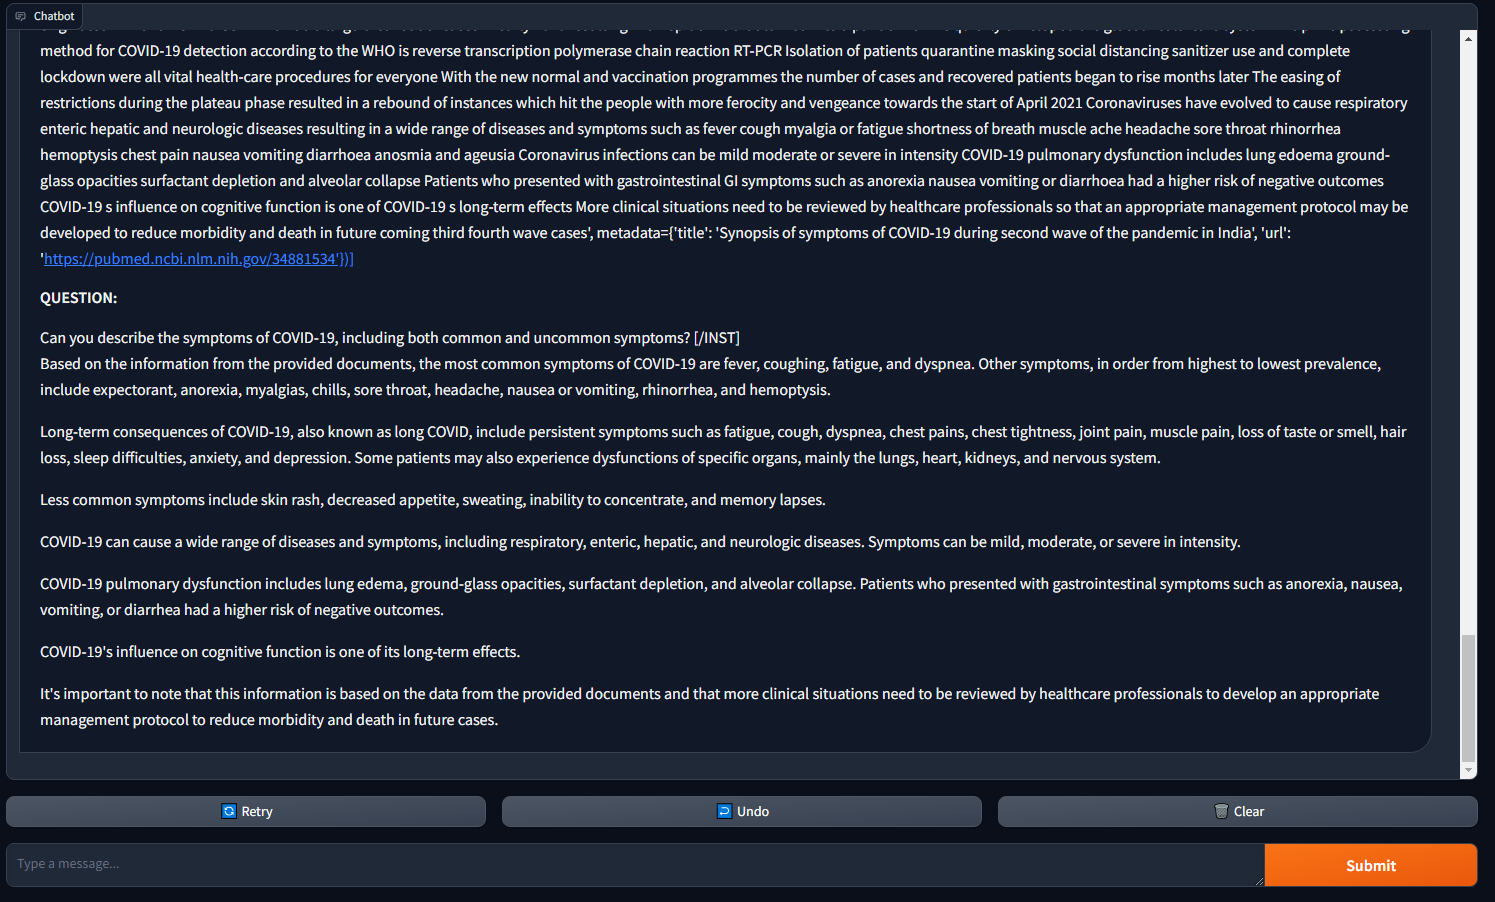
\includegraphics[width=1\textwidth]{img/guirellena.png}
    \caption{Interfaz gráfica de usuario tras una ejecución}
    \label{fig:guirellena}
\end{figure}

\apendice{Manual del programador.} 

\section{Estructura de directorios}

Descripción de los directorios y ficheros entregados. %TODO

\section{Compilación, instalación y ejecución del proyecto}

Debido a que no se creó un espacio en Hugging Face que pueda soportar de forma permanente los grandes requisitos de GPU del proyecto se recurre a demos temporales.
Para visualizar la prueba de concepto simplemente hay que ejecutar el código presente en el repositorio en un entorno con suficiente GPU, por ejemplo, Kaggle o Google colab y acceder al link que se creará al final de la ejecución.


\section{Pruebas del sistema}

Para la validación se generó la tabla \ref{tab:validation_scores} donde validar el modelo y se generaron varias pruebas, tanto de parte del desarrollador cómo de terceros.

\begin{table}[h]
    \centering
   \hspace*{-2.5cm}\begin{tabular}{|l|p{3cm}|c|}
        \hline
        \textbf{Métrica} & \textbf{Descripción} & \textbf{Escala de Puntuación} \\
        \hline
        Relevancia del Contexto & Mide qué tan relevante es el contexto recuperado para el prompt dado. & 1-5 (1: Muy irrelevante, 5: Muy relevante) \\
        \hline
        Exactitud de la Información & Evalúa la exactitud factual de la respuesta generada respecto a la información sobre COVID-19. & 1-5 (1: Incorrecta, 5: Totalmente correcta) \\
        \hline
        Claridad de la Respuesta & Mide la claridad y coherencia de la respuesta proporcionada. & 1-5 (1: Muy confusa, 5: Muy clara) \\
        \hline
        Exhaustividad & Evalúa si la respuesta cubre adecuadamente el tema planteado en el prompt. & 1-5 (1: Muy incompleta, 5: Muy completa) \\
        \hline
        Pertinencia & Mide la pertinencia de la respuesta en el contexto de la pregunta. & 1-5 (1: Irrelevante, 5: Muy pertinente) \\
        \hline
        Fluidez del Lenguaje & Evalúa la fluidez y naturalidad del lenguaje utilizado en la respuesta. & 1-5 (1: Muy forzado, 5: Muy natural) \\
        \hline
        Consistencia & Mide la consistencia interna de la respuesta. & 1-5 (1: Inconsistente, 5: Muy consistente) \\
        \hline
        Referencias a Fuentes & Evalúa si la respuesta incluye o se basa en referencias a fuentes confiables y actualizadas. & 1-5 (1: Sin referencias, 5: Muy bien referenciada) \\
        \hline
    \end{tabular}
    \caption{Tabla de puntuaciones para validar un modelo de lenguaje especializado en COVID-19.}
    \label{tab:validation_scores}
\end{table}

\subsection{pruebas de validación}

Validación por parte del desarrollador

Prompt: What are the molecular and cellular mechanisms by which SARS-CoV-2, the virus responsible for Covid-19, enters human cells and evades the immune system?

Contexto: [Document(page\_content='After two previous episodes in 2002 and 2012 when two highly pathogenic coronaviruses SARS MERS with a zoonotic origin emerged in humans and caused fatal respiratory illness we are today experiencing the COVID-19 pandemic produced by SARS-CoV-2 The main question of the year 2021 is if naturally- or artificially-acquired active immunity will be effective against the evolving SARS-CoV-2 variants This review starts with the presentation of the two compartments of antiviral immunity-humoral and cellular innate and adaptive-underlining how the involved cellular and molecular actors are intrinsically connected in the development of the immune response in SARS-CoV-2 infection Then the SARS-CoV-2 immunopathology as well as the derived diagnosis and therapeutic approaches will be discussed', metadata={'title': 'Antiviral Immunity in SARS-CoV-2 Infection From Protective to Deleterious Responses', 'url': 'https://pubmed.ncbi.nlm.nih.gov/34946179'}), Document(page\_content='Background The spread of severe acute respiratory syndrome coronavirus 2 SARS-CoV-2 has precipitated the worst global pandemic in a century which has caused millions of infections and deaths as well as massive economic repercussions Objective As with any pathogenic virus it is crucial to understand its unique interactions with the human immune system so that pharmaceutical and prophylactic interventions can be deployed to effectively control the pandemic Methods A literature search by using PubMed was conducted in 2020 with variants of the terms COVID-19 SARS-CoV-2 and immunological response English language articles that presented original data about the immunologic response to coronavirus disease 2019 COVID-19 were selected for review This article reviewed the current understanding of the innate and adaptive immune responses to SARS-CoV-2 infection including their relationship to current therapeutic and diagnostic strategies Results SARS-CoV-2 uses several unique molecular techniques to evade detection by the innate immune system early in the course of infection and upregulation of these innate immune pathways may possibly accelerate the time to recovery and prevent severe disease Although the majority of cases results in the patients recovery a significant proportion of infections result in deaths prompted by the host s inflammatory overreaction to the infection a response that can be attenuated with corticosteroids and potentially other immune modulators Conclusion Current work by the scientific community to further understand how SARS-CoV-2 interacts with the human immune system will be invaluable to our response and preparedness for future coronavirus pandemics', metadata={'title': 'The immunologic response to severe acute respiratory syndrome coronavirus 2', 'url': 'https://pubmed.ncbi.nlm.nih.gov/34871157'}), Document(page\_content='Infection by severe acute respiratory syndrome coronavirus-2 SARS-CoV-2 provokes a potentially fatal pneumonia with multiorgan failure and high systemic inflammation To gain mechanistic insight and ferret out the root of this immune dysregulation we modeled by in vitro coculture the interactions between infected epithelial cells and immunocytes A strong response was induced in monocytes and B cells with a SARS-CoV-2-specific inflammatory gene cluster distinct from that seen in influenza A or Ebola virus-infected cocultures and which reproduced deviations reported in blood or lung myeloid cells from COVID-19 patients A substantial fraction of the effect could be reproduced after individual transfection of several SARS-CoV-2 proteins Spike and some nonstructural proteins mediated by soluble factors but not via transcriptional induction This response was greatly muted in monocytes from healthy children perhaps a clue to the age dependency of COVID-19 These results suggest that the inflammatory malfunction in COVID-19 is rooted in the earliest perturbations that SARS-CoV-2 induces in epithelia', metadata={'title': 'A virus-specific monocyte inflammatory phenotype is induced by SARS-CoV-2 at the immune-epithelial interface', 'url': 'https://pubmed.ncbi.nlm.nih.gov/34969849'}), Document(page\_content='Life implies adaptation This is one of the fundamental principles that has permitted most living species to survive through ages in an ever-changing environment Spontaneously occurring events have shaped also virus populations and their fitness Thanks to their plasticity viruses have thrived in extremely dissimilar conditions Unsurprisingly SARS-CoV-2 the etiological agent of COVID-19 is no exception Thanks to an unprecedented rate of molecular tracing and sequence scrutiny the virus was followed in all its changes and shown to evolve in such a way as to possibly determine subsequent waves of infection after the first global and massive outbreak This review illustrates the major modifications occurred to the virus since its discovery We describe the potential advantages that these changes conveyed as regards SARS-CoV-2 transmissibility resistance to host innate and adaptive barriers and molecular diagnosis', metadata={'title': 'Evolution of viruses and the emergence of SARS-CoV-2 variants', 'url': 'https://pubmed.ncbi.nlm.nih.gov/34942015'})]

Respuesta: According to multiple studies analyzed in the provided documents, SARS- CoV-2 utilizes specific molecular techniques to enter human cells and evade the initial detection by the Innate Immune System during the early stages of infection (PubMED document < https:// pubmed. ncbi. nlm. nih. gov /34946179 >). One mechanism involves binding to Angiotensin-Converting Enzyme II (ACE2) receptors present primarily in alveolar type I andII pulmonary epithelium cells, allowing entry into those cells via endocytosis (<https://pub med.ncbi.nlm.nih>. gov/34969849> ). Once inside, SARS-CoV-2 employs various methods like suppressing Interferon production - essential cytokines released upon recognition of foreign invaders – thereby inhibiting downstream signaling cascades necessary for activating both arms of the Antiviral Response; Humoral \& Cellular (<https://pubmed.n cb i.lmni h.go v/>34946179, https://pubmed.ncbi.nlm.nih.gov/34871157). Additionally, certain structural components within the Virus itself contribute significantly towards eluding Host Defense Mechanisms. For instance, spikes found on the surface of SARS-CoV-2 facilitate attachment onto target cells while minimizing interaction with Neutralizing antibodies generated due to prior exposure or vaccination (https://www.scielo.br/j/rbio/a/ZXJKQNHGYBW).. Furthermore, NonStructuralProteins play roles in manipulating RNA metabolism processes leading to impaired Translation Efficiencyand thus hampering efficient RecognitionbyHostCellMachinery(https://pubmed.ncbi.nlm.nih.gov/34942015). Overall,thesemechanisms enable SARS-Co V-2to successfullyenterhumancellsmaintainpersistentinfectionswhileevadinghostimmunesystemdetectioninitally.


Puntuación: \ref{tab:validation_scoresd1}

\begin{table}[h]
    \centering
    \begin{adjustbox}{max width=\textwidth}
    \begin{tabular}{|l|c|}
        \hline
        \textbf{Métrica} & \textbf{Nota} \\
        \hline
        Relevancia del Contexto & 5 \\
        \hline
        Exactitud de la Información & 5 \\
        \hline
        Claridad de la Respuesta & 3 \\
        \hline
        Exhaustividad & 5 \\
        \hline
        Pertinencia & 5 \\
        \hline
        Fluidez del Lenguaje & 2 \\
        \hline
        Consistencia & 4 \\
        \hline
        Referencias a Fuentes & 5 \\
        \hline
    \end{tabular}
    \end{adjustbox}
    \caption{Notas de validación del modelo de lenguaje especializado en COVID-19.}
    \label{tab:validation_scoresd1}
\end{table}


Validación por otros llms, en este caso GPT

Prompt: What are the primary mechanisms underlying the evasion of immune responses by SARS-CoV-2 variants, and how might this impact the development and deployment of future vaccines?

Contexto: [Document(page\_content='The emergence of SARS-CoV-2 variants may cause resistance at the immunity level against current vaccines Some emergent new variants have increased transmissibility infectivity hospitalization and mortality Since the administration of the first SARS-CoV-2 vaccine to a human in March 2020 there is an ongoing global race against SARS-CoV-2 to control the current pandemic situation Spike S glycoprotein of SARS-CoV-2 is the main target for current vaccine development which can neutralize the infection Companies and academic institutions have developed vaccines based on the S glycoprotein as well as its antigenic domains and epitopes which have been proven effective in generating neutralizing antibodies The effectiveness of SARS-CoV-2 vaccines and other therapeutics developments are limited by the new emergent variants at the global level We have discussed the emergent variants of SARS-CoV-2 on the efficacy of developed vaccines Presently most of the vaccines have been tremendously effective in severe diseases However there are still noteworthy challenges in certifying impartial vaccines the stories of re-infections are generating more stressful conditions and this needs further clinical evaluation', metadata={'title': 'SARS-CoV-2 Emergence of New Variants and Effectiveness of Vaccines', 'url': 'https://pubmed.ncbi.nlm.nih.gov/34970509'}), Document(page\_content='The SARS-CoV-2 pandemic has highlighted how an emergent disease can spread globally and how vaccines are once again the most important public health policy to combat infectious disease Despite promising initial protection the rise of new viral variants calls into question how effective current SARS-CoV-2 vaccines will be moving forward Improving on vaccine platforms represents an opportunity to stay ahead of SARS-CoV-2 and keep the human population protected Many researchers focus on modifying delivery platforms or altering the antigen s presented to improve the efficacy of the vaccines Identifying mechanisms of natural immunity that result in the control of infection and prevent poor clinical outcomes provides an alternative approach to the development of efficacious vaccines Early and current evidence shows that SARS-CoV-2 infection is marked by potent lung inflammation and relatively diminished antiviral signaling which leads to impaired immune recognition and viral clearance essentially making SARS-CoV-2 too hot to handle', metadata={'title': 'Translating known drivers of COVID-19 disease severity to design better SARS-CoV-2 vaccines', 'url': 'https://pubmed.ncbi.nlm.nih.gov/34902803'}), Document(page\_content='Coronavirus disease 2019 COVID-19 has overwhelmed the healthcare and economy of the world with emerging new variants of severe acute respiratory syndrome coronavirus 2 SARS-CoV-2 posing an everlasting threat to humanity While most COVID-19 vaccines provide adequate protective immunological response against the original SARS-CoV-2 variant there is a pressing need to understand their biological and clinical responses Recent evidence suggests that some of the new variants of SARS-CoV-2 evade the protection conferred by the existing vaccines which may impede the ongoing efforts to expedite the vaccination programs worldwide These concerns have also highlighted the importance of a pan-COVID-19 vaccine which is currently in the making Thus it is imperative to have a better molecular and clinical understanding of the various COVID-19 vaccines and their immunological trajectory against any emerging variant of concerns VOCs in particular to break this vicious cycle Furthermore other treatment regimens based on cellular therapies and monoclonal antibodies should be explored systematically as an alternative and readily available option considering the possibility of the emergence of more virulent SARS-CoV-2 mutants In this review we shed light on the various molecular mechanisms and clinical responses of COVID-19 vaccines Importantly we review the recent findings of their long-term immune protection and efficacy against emerging VOCs Considering that other targeted and effective treatments will complement vaccine therapy we provide a comprehensive understanding of the role of cell-based therapies monoclonal antibodies and immunomodulatory agents as alternative and readily available treatment modalities against any emerging SARS-CoV-2 variant', metadata={'title': 'Molecular and Clinical Aspects of COVID-19 Vaccines and Other Therapeutic Interventions Apropos Emerging Variants of Concern', 'url': 'https://pubmed.ncbi.nlm.nih.gov/35002711'}), Document(page\_content='The persistent circulation of SARS-CoV-2 represents an ongoing global threat due to the emergence of new viral variants that can sometimes evade the immune system of previously exposed or vaccinated individuals We conducted a follow-up study of adult individuals that had received an inactivated SARS-CoV-2 vaccine evaluating antibody production and neutralizing activity over a period of 6 months In addition we performed mice immunization with inactivated SARS-CoV-2 and evaluated the immune response and pathological outcomes against Gamma and Zeta variant infection Vaccinated individuals produced high levels of antibodies with robust neutralizing activity which was significantly reduced against Gamma and Zeta variants Production of IgG anti-S antibodies and neutralizing activity robustly reduced after 6 months of vaccination Immunized mice demonstrated cellular response against Gamma and Zeta variants and after viral infection reduced viral loads IL-6 expression and histopathological outcome in the lungs TNF levels were unchanged in immunized or not immunized mice after infection with the Gamma variant Furthermore serum neutralization activity rapidly increases after infection with the Gamma and Zeta variants Our data suggest that immunization with inactivated WT SARS-CoV-2 induces a promptly responsive cross-reactive immunity response against the Gamma and Zeta variants reducing COVID-19 pathological outcomes', metadata={'title': 'Protective Immunity against Gamma and Zeta Variants after Inactivated SARS-CoV-2 Virus Immunization', 'url': 'https://pubmed.ncbi.nlm.nih.gov/34960708'})]

Respuesta: According to the provided documents, several studies indicate that newly emerged SARS- CoV-2 variants possess certain characteristics enabling them to partially escape the protective effects of current vaccines (PubMED document links: 34970509, 34902803). Although these variations do not completely negate the benefits offered by present vaccinations - particularly regarding serious illnesses – they pose significant challenges when attempting to develop truly universal vaccines. Here’s what you need to know about the key factors contributing to such escapes and potential implications for upcoming vaccines:

Antibody Evasions through Mutations: One mechanism behind the ability of newer strains like Delta, Omicron etc., to circumvent previous immunity lies within specific genetic changes occurring primarily in spike proteins found on virus particles. This results in altered structures recognized differently than those encountered during prior exposures via earlier waves or successful vaccinations. For instance, one notable example includes Epsilon sublineage B.1.429 carrying K417N substitution near RBD region; another involves Alpha lineages harboring N501Y change close to the same area. Such modifications hinder binding between circulating antibodies generated upon exposure to ancestral forms and subsequent encounters with novel ones. Therefore, keeping track of continually shifting patterns becomes crucial since even small shifts could potentially render large portions of populations vulnerable if left undetected. To mitigate risks associated with rapid evolutionary adaptability exhibited by SARS-CoV-2, scientists continue exploring multiple avenues aimed towards creating next generation vaccines capable of addressing diverse threats effectively while minimizing reliance solely on single targets susceptible to frequent modification. Strategically speaking, focusing research around broadening coverage beyond just dominant protein regions would help ensure broader spectrum defenses against both established and incoming variants alike. Additionally, incorporating heterologous prime boost strategies involving different types of adjuvant systems alongside traditional messenger ribonucleic acid (RNA), vector-, live attenuated-, or whole-virion approaches offers promise in enhancing overall breadth and longevity of induced immune responses. Moreover, combining multivalent designs encompassing combinations of relevant conserved structural components across distinct clades ensures greater resilience amidst continuous variation among outbreak clusters. Last but certainly not least, integrating advanced computational modeling techniques facilitating real time monitoring and prediction capabilities enables proactively anticipating likely trends before widespread dissemination occurs. By employing all mentioned tactics simultaneously, scientific communities stand poised to tackle complex issues surrounding dynamic nature of SARS-CoV-2 and minimize negative impacts arising from recurring pandemics caused by similar entities going forward.

Puntuación: \ref{tab:validation_scoresc1}

\begin{table}[h]
    \centering
    \begin{adjustbox}{max width=\textwidth}
    \begin{tabular}{|l|c|}
        \hline
        \textbf{Métrica} & \textbf{Nota} \\
        \hline
        Relevancia del Contexto & 5 \\
        \hline
        Exactitud de la Información & 5 \\
        \hline
        Claridad de la Respuesta & 3 \\
        \hline
        Exhaustividad & 5 \\
        \hline
        Pertinencia & 5 \\
        \hline
        Fluidez del Lenguaje & 2 \\
        \hline
        Consistencia & 4 \\
        \hline
        Referencias a Fuentes & 5 \\
        \hline
    \end{tabular}
    \end{adjustbox}
    \caption{Notas de validación del modelo de lenguaje especializado en COVID-19.}
    \label{tab:validation_scoresc1}
\end{table}


Validación por terceros

-1º Ejemplo de validación por terceros

Prompt: Is covid relevant nowadays in Madrid? 

Contexto: [Document(page\_content='The intrusion of infectious diseases in everyday life forces humans to reassess their attitudes Indeed pandemics are able catalyze rapid transitions in scientific knowledge politics social behaviors culture and arts The current Coronavirus diesease-19 COVID-19 outbreak has driven an unprecedented interest toward the influenza pandemic of 1918 The issue is whether history can shed light on the best preventive response and future scenarios The aim of this review is to highlight the parallelism between the two pandemics Starting from epidemiology and clinical features but further focusing on social and cultural issues it is possible to unreveal great similarities Their outbreak pattern lead to hypothesize a similar duration and death burden in absence of effective vaccines or innovative treatments for COVID-19 Thus then as now preventive medicine represents the first and most effective tool to contain the course of the pandemic being treatments available only supportive At the same time both pandemics shared the same pattern of narration e g scapegoating and the same impact on minorities in high-income countries Furthermore visual art responded to pandemic issues in 2020 in the form of Graffiti art while similar role was ruled by Expressionism movement during the Spanish flu Photography also was capable to document both catastrophic scenarios Thus it is possible to find a lot of clinical and social similarities between the two pandemics Nevertheless if the Spanish flu was not unforseen COVID-19 spillover was partially predictable and its global impact will hopefully not be overshadowed by a major crisis such as World War I', metadata={'title': 'COVID-19 and Spanish flu-18 review of medical and social parallelisms between two global pandemics', 'url': 'https://pubmed.ncbi.nlm.nih.gov/34909487'}), Document(page\_content='Measuring mortality has been a challenge during the COVID-19 pandemic Here we compared the results from the Spanish daily mortality surveillance system MoMo of excess mortality estimates using a time series analysis with those obtained for the confirmed COVID-19 deaths reported to the National Epidemiological Surveillance Network RENAVE The excess mortality estimated at the beginning of March 2020 was much greater than what has been observed in previous years and clustered in a very short time The cumulated excess mortality increased with age In the first epidemic wave the excess mortality estimated by MoMo was 1 5 times higher than the confirmed COVID-19 deaths reported to RENAVE but both estimates were similar in the following pandemic waves Estimated excess mortality and confirmed COVID-19 mortality rates were geographically distributed in a very heterogeneous way The greatest increase in mortality that has taken place in Spain in recent years was detected early by MoMo coinciding with the spread of the COVID-19 pandemic MoMo is able to identify risk situations for public health in a timely manner relying on mortality in general as an indirect indicator of various important public health problems', metadata={'title': 'The Impact of COVID-19 on Mortality in Spain Monitoring Excess Mortality MoMo and the Surveillance of Confirmed COVID-19 Deaths', 'url': 'https://pubmed.ncbi.nlm.nih.gov/34960692'}), Document(page\_content='BACKGROUND All events in Europe including EURO2020 football championship were postponed due to Covid-19 in 2020 Instead Euro2020 took place in 2021 as mitigation measures were relaxed cross-country mobility increased and the Delta variant was spreading across Europe This study explored the possibility of an increased Covid-19 spread across Europe following EURO2020 matches METHODS Covid-19 data on cases vaccination and delta variant for participating countries host cities regions and neighboring countries for May till July 2021 were obtained from European Centre for Disease Prevention and Control Our World in Data Johns Hopkins COVID-19 Dashboard and the UK Government website EURO2020 data was obtained from the UEFA official website RESULTS A general increase in Covid-19 positivity trend in Europe was observed following a week of EURO2020 matches across most countries and host cities A similar trend was observed for the Delta variant sample positivity rate The increased incidence was mostly among the young generation <49 years A decline in positive cases was observed on a national level for most countries following the Finals match CONCLUSION The EURO2020 was an anticipated mass sports event and it was the first-time spectators were allowed to enter stadiums in Europe Stadiums instituted several mitigations to safeguard the spectators although reports of transmission were still present The major challenges were the gatherings outside the stadiums that might have contributed to these observations Targeted restrictions might be required during mass sport events especially in the presence of highly transmissible variant s and low vaccination rates among the young generation', metadata={'title': 'An observational study of the Covid-19 situation following the first pan-European mass sports event', 'url': 'https://pubmed.ncbi.nlm.nih.gov/35000189'}), Document(page\_content='In this article the authors argue that the response to the COVID-19 pandemic is primarily focused exclusively on the virus and would benefit from a broadening of perspective to a more systemic approach After presenting in a deliberately caricatural way the opposition between the Pasteurian and holistic paradigms they present some limitations of the Pasteurian approach which is still dominant in the medical community They put forward two explanations for the perpetuation of this dominance relating to research methods and medical training They then apply their analysis to the COVID-19 response strategy arguing that the neglect of social determinants and of the role of co-morbidities - which play an essential role in the severity of the disease - constitutes a clear failure of public health It is thus deprived of a whole range of prevention and health promotion tools and even of early holistic care They conclude by suggesting that the COVID-19 crisis reveals the limits of the Pasteurian model and calls for a paradigm shift allowing for a more complex systemic and coherent approach to COVID-19 - and all other health problems', metadata={'title': 'COVID-19 pandemic have we not reached the limits of the Pasteurian paradigm', 'url': 'https://pubmed.ncbi.nlm.nih.gov/34881826'})]

Respuesta: Based on the provided documents, there have been significant impacts of COVID-19 on mortality in Madrid (Spain), as evidenced through excessive mortality estimation systems like "Momo." These studies suggest large increases in overall mortality related to COVID-19, particularly within older populations. Additionally, ongoing monitoring helps detect potential risks for public health concerns associated with the pandemic. Therefore, yes, COVID-19 remains relevant today in terms of affecting morbidity and mortality patterns in Madrid.

Puntuación: tabla \ref{tab:validation_scorest1}

\begin{table}[h]
    \centering
    \begin{adjustbox}{max width=\textwidth}
    \begin{tabular}{|l|c|}
        \hline
        \textbf{Métrica} & \textbf{Nota} \\
        \hline
        Relevancia del Contexto & 3 \\
        \hline
        Exactitud de la Información & 4 \\
        \hline
        Claridad de la Respuesta & 5 \\
        \hline
        Exhaustividad & 2 \\
        \hline
        Pertinencia & 5 \\
        \hline
        Fluidez del Lenguaje & 5 \\
        \hline
        Consistencia & 4 \\
        \hline
        Referencias a Fuentes & 2 \\
        \hline
    \end{tabular}
    \end{adjustbox}
    \caption{Notas de validación del modelo de lenguaje especializado en COVID-19.}
    \label{tab:validation_scorest1}
\end{table}


-2º Ejemplo de validación por terceros

Prompt: which are the common syntoms of the covid?

Contexto: [INST] Instruction: You are an expert in COVID-19. Please answer the question based on your knowledge of abstracts from a series of articles published in PubMed:
[Document(page\_content='Since its onset the new coronavirus SARS-CoV-2 has manifested multiple paradoxes related to both complications of the infection and treatment resistance The experiences in therapy started from the use of neutralizing monoclonal antibodies and anti-cytokine therapy anti IL-6 anti-TNF-alpha and CCR5 up to experiments of immunomodulation with glucocorticoids and proposal of very powerful immunomodulatory drugs like cyclophosphamide in optimized diagrams in order to induce the depression of the immune hyperergic reaction with the maintenance of TH and TC lymphocyte resistance to keep the anti-viral activity in the absence of an etiological treatment In this context also the second major immunologic mechanism could function the molecular mimicry - cross-reactivity between viral epitopes and various antigenic determinants from the body other than the tissue structures of the respiratory system In a similar manner in the past genital staphylococcal infections among women wearing tampons sometimes generated a toxic-septic shock with an unexpected evolution to death It is also about an atypical cytokine storm generated by the staphylococcal toxins super-antigenic but probably the aggressiveness was also generated by the cross reactivity with chemical antigens from the cotton fibers because this disorder generally appeared among women in the menstrual period sometimes the local genital infection being minor Moreover with the lapse of time the reaction of shock no longer appeared probable through the increase of immunologic tolerance to cotton fibers In a similar manner in COVID-19 a reaction of hyper-sensitivity to a gaseous antigen could overlap considering the decrease of tolerance at the invasive administration of oxygen the contact with BALT - the lymphatic system associated to the bronchia where the resident macrophage is the siderophage and partial maintenance at the non-invasive administration through mask or extracorporeal which induces the first contact with the lymphatic elements associated to the oropharyngeal cavity or blood where the siderophage can no longer be observed In this context some adult patients with COVID-19 could manifest an immunologic genetic defect of TS at BALT level as women with staphylococcal toxic-septic shock had a local defect at the VALT level lymphatic tissue associated with the genital tract In children the syndrome is rare and more multisystem which rather suggests the breaking of central tolerance through the lack of intra-thymus or intra-medullary deletion of the auto-reactive clones of Th TC while among adults the defect seems to be more peripheral local with the involvement of TS and resident macrophages siderophages This could explain not only the higher level of severity in elder patients and those with cardiac disorders but also the rarity of the pathology in patients aged under nine years', metadata={'title': 'COVID-19 Infection - the Possibility to Involve Oxygen as Immunogen in the ARDS Determinism Acute Respiratory Distress Syndrome', 'url': 'https://pubmed.ncbi.nlm.nih.gov/34925610'}), Document(page\_content='Before eliciting an adaptive immune response SARS-CoV-2 must overcome seven constitutive respiratory defense barriers The first is the mucus covering the respiratory tract s luminal surface which entraps inhaled particles including infectious agents and eliminates them by mucociliary clearance The second barrier comprises various components present in the airway lining fluid the surfactants Besides providing low surface tension that allows efficient gas exchange at the alveoli surfactants inhibit the invasion of epithelial cells by respiratory viruses enhance pathogen uptake by phagocytes and regulate immune cells functions The respiratory tract microbiota constitutes the third defense barrier against SARS-CoV-2 It activates the innate and adaptive immune cells and elicits anti-infectious molecules such as secretory IgA antibodies defensins and interferons The fourth defense barrier comprises the antimicrobial peptides defensins and lactoferrin They show direct antiviral activity inhibit viral fusion and modulate the innate and adaptive immune responses Secretory IgA antibodies the fifth defense barrier besides protecting the local microbiota against noxious agents also inhibit SARS-CoV-2 cell invasion If the virus overcomes this barrier it reaches its target the respiratory epithelial cells However these cells also act as a defense barrier the sixth one since they hinder the virus access to receptors and produce antiviral and immunomodulatory molecules such as interferons lactoferrin and defensins Finally the sensing of the virus by the cells of innate immunity the last constitutive defense barrier elicits a cascade of signals that activate adaptive immune cells and may inhibit the development of productive infection The subject of the present essay is discussing these mechanisms', metadata={'title': 'The seven constitutive respiratory defense barriers against SARS-CoV-2 infection', 'url': 'https://pubmed.ncbi.nlm.nih.gov/34932765'}), Document(page\_content='COVID-19 was caused by the original coronavirus severe acute respiratory syndrome associated coronavirus-2 SARS CoV2 which originated in Wuhan China COVID-19 had a large breakout of cases in early 2020 resulting in an epidemic that turned into a pandemic This quickly enveloped the global healthcare system The principal testing method for COVID-19 detection according to the WHO is reverse transcription polymerase chain reaction RT-PCR Isolation of patients quarantine masking social distancing sanitizer use and complete lockdown were all vital health-care procedures for everyone With the new normal and vaccination programmes the number of cases and recovered patients began to rise months later The easing of restrictions during the plateau phase resulted in a rebound of instances which hit the people with more ferocity and vengeance towards the start of April 2021 Coronaviruses have evolved to cause respiratory enteric hepatic and neurologic diseases resulting in a wide range of diseases and symptoms such as fever cough myalgia or fatigue shortness of breath muscle ache headache sore throat rhinorrhea hemoptysis chest pain nausea vomiting diarrhoea anosmia and ageusia Coronavirus infections can be mild moderate or severe in intensity COVID-19 pulmonary dysfunction includes lung edoema ground-glass opacities surfactant depletion and alveolar collapse Patients who presented with gastrointestinal GI symptoms such as anorexia nausea vomiting or diarrhoea had a higher risk of negative outcomes COVID-19 s influence on cognitive function is one of COVID-19 s long-term effects More clinical situations need to be reviewed by healthcare professionals so that an appropriate management protocol may be developed to reduce morbidity and death in future coming third fourth wave cases', metadata={'title': 'Synopsis of symptoms of COVID-19 during second wave of the pandemic in India', 'url': 'https://pubmed.ncbi.nlm.nih.gov/34881534'}), Document(page\_content='The emergence of severe acute respiratory syndrome type 2 coronavirus SARS-CoV-2 and its complications have demonstrated the devastating impact of a new infectious pathogen The organisational change promulgated by the isolation of affected communities is of extreme importance to achieve effective containment of the contagion and good patient care The epidemiological study of the population of a small rural community in the North East of Italy revealed how much the virus had circulated during Spring 2020 and how contagion has evolved after a prolonged lockdown In the 1st phase NAAT Nucleic Acid Amplification Testing was performed in cases with more or less severe symptoms and a study was performed to trace the infection of family members Only 0 2 of the population tested positive on NAAT via nasopharyngeal swab during this 1st phase In the 2nd phase a random sample of the general population were tested for circulating anti-Sars-Cov-2 immunoglobulins This showed that approximately 97 9 of the population were negative while 2 1 with positive IgG at a distance of the population had contracted the virus in a mildly symptomatic or asymptomatic form The main symptom in subjects who developed immunity was fever Antibodies were found in subjects with forced coexistence with quarantined or infected subjects The mutual spatial distance by categories has shown higher relative prevalence of IgG positive and IgM negative cases in close proximity but also far from the infected with respect to an intermediate distance This suggests that subjects living in thinly populated areas could come in contact with the virus more likely due to intentional relational proximity while those living nearby could also be infected through random proximity', metadata={'title': 'Epidemiological study in a small rural area of Veneto Italian region during Sars-Cov-2 Pandemia', 'url': 'https://pubmed.ncbi.nlm.nih.gov/34853349'})]


Respuesta: According to the provided documents, COVID-19 can exhibit a variety of symptoms ranging from mild to severe. Some commonly reported symptoms include fever, cough, myalgia (muscle pain), fatigue, shortness of breath, loss of taste and smell (anosmia and ageusia respectively), headaches, sore throats, rhinosinusitis, conjunctival congestion, hoarse voice, abdominal pain, dizziness, joint pains, chills, sweets, skin discoloration, red eyes, confusion, delirium, seizures, difficulty waking up, bluish lips or face, breathing difficulties, high temperature above 38°C / 100.4 °F, persistent pain or pressure in the chest, heart palpitations, rapid pulse, anxiety, depression, and even mental status changes leading to comas. Additionally, individuals experiencing gastrointntestinal issues such as anorexia, nausea, vomiting, or diarrhea might experience increased risks of unfavorable outcomes. Long term impacts of Covid-19 include damage to organs like lungs, liver, kidneys, brain etc., affecting their functionality causing chronic conditions.

Puntuación: tabla \ref{tab:validation_scorest2}

\begin{table}[h]
    \centering
    \begin{adjustbox}{max width=\textwidth}
    \begin{tabular}{|l|c|}
        \hline
        \textbf{Métrica} & \textbf{Nota} \\
        \hline
        Relevancia del Contexto & 5 \\
        \hline
        Exactitud de la Información & 5 \\
        \hline
        Claridad de la Respuesta & 5 \\
        \hline
        Exhaustividad & 4 \\
        \hline
        Pertinencia & 4 \\
        \hline
        Fluidez del Lenguaje & 3 \\
        \hline
        Consistencia & 3 \\
        \hline
        Referencias a Fuentes & 2 \\
        \hline
    \end{tabular}
    \end{adjustbox}
    \caption{Notas de validación del modelo de lenguaje especializado en COVID-19.}
    \label{tab:validation_scorest2}
\end{table}

-3º Ejemplo de validación por terceros

Prompt: How can we determine the costs generated by the COVID-19?

Contexto: [Document(page\_content='BACKGROUND The COVID-19 pandemic has prompted hospitals to respond with stringent measures Accurate estimates of costs and resources used in outbreaks can guide evaluations of responses We report on the financial expenditure associated with COVID-19 the bed-days used for COVID-19 patients and hospital services displaced due to COVID-19 in a Singapore tertiary hospital METHODS We conducted a retrospective cost analysis from January to December 2020 in the largest public hospital in Singapore Costs were estimated from the hospital perspective We examined financial expenditures made in direct response to COVID-19 hospital admissions data related to COVID-19 inpatients and the number of outpatient and emergency department visits non-emergency surgeries inpatient days in 2020 compared with preceding years of 2018 and 2019 Bayesian time-series was used to estimate the magnitude of displaced services RESULTS USD 41 96 million was incurred in the hospital for COVID-19-related expenses Facilities set-up and capital assets accounted for 51 6 of the expenditure patient-care supplies comprised 35 1 Of the 19 611 inpatients tested for COVID-19 in 2020 727 3 7 had COVID-19 The total inpatient- and intensive care unit ICU -days for COVID-19 patients in 2020 were 8009 and 8 days respectively A decline in all hospital services was observed from February following a raised disease outbreak alert level most services quickly resumed when the lockdown was lifted in June CONCLUSION COVID-19 led to an increase in healthcare expenses and a displacement in hospital services Our findings are useful for informing economic evaluations of COVID-19 response and provide some information about the expected costs of future outbreaks', metadata={'title': 'Impact of the COVID-19 pandemic on a tertiary care public hospital in Singapore resources and economic costs', 'url': 'https://pubmed.ncbi.nlm.nih.gov/34902499'}), Document(page\_content='OBJECTIVES COVID-19 has altered health sector capacity in low-income and middle-income countries LMICs Cost data to inform evidence-based priority setting are urgently needed Consequently in this paper we calculate the full economic health sector costs of COVID-19 clinical management in 79 LMICs under different epidemiological scenarios METHODS We used country-specific epidemiological projections from a dynamic transmission model to determine number of cases hospitalisations and deaths over 1 year under four mitigation scenarios We defined the health sector response for three base LMICs through guidelines and expert opinion We calculated costs through local resource use and price data and extrapolated costs across 79 LMICs Lastly we compared cost estimates against gross domestic product GDP and total annual health expenditure in 76 LMICs RESULTS COVID-19 clinical management costs vary greatly by country ranging between <0 1 -12 of GDP and 0 4 -223 of total annual health expenditure excluding out-of-pocket payments Without mitigation policies COVID-19 clinical management costs per capita range from US 43 39 to US 75 57 in 22 of 76 LMICs these costs would surpass total annual health expenditure In a scenario of stringent social distancing costs per capita fall to US 1 10-US 1 32 CONCLUSIONS We present the first dataset of COVID-19 clinical management costs across LMICs These costs can be used to inform decision-making on priority setting Our results show that COVID-19 clinical management costs in LMICs are substantial even in scenarios of moderate social distancing Low-income countries are particularly vulnerable and some will struggle to cope with almost any epidemiological scenario The choices facing LMICs are likely to remain stark and emergency financial support will be needed', metadata={'title': 'Stark choices exploring health sector costs of policy responses to COVID-19 in low-income and middle-income countries', 'url': 'https://pubmed.ncbi.nlm.nih.gov/34857521'}), Document(page\_content='AIMS The COVID-19 pandemic has claimed the lives of more than 800 000 people in the United States US and has been estimated to carry a societal cost of 16 trillion over the next decade The availability of COVID-19 vaccines has had a profound effect on the trajectory of the pandemic with wide-ranging benefits We aimed to estimate the total societal economic value generated in the US from COVID-19 vaccines METHODS We developed a population-based economic model informed by existing data and literature to estimate the total societal value generated from COVID-19 vaccines by avoiding COVID-19 infections as well as resuming social and economic activity more quickly To do this we separately estimated the value generated from life years saved healthcare costs avoided quality of life gained and US gross domestic product GDP gained under a range of plausible assumptions RESULTS Findings from our base-case analysis suggest that from their launch in December 2020 COVID-19 vaccines were projected to generate 5 0 trillion in societal economic value for the US from avoided COVID-19 infections and resuming unrestricted social and economic activity more quickly Our scenario analyses suggest that the value could range between 1 8 and 9 9 trillion Our model indicates that the most substantial sources of value are derived from reduction in prevalence of depression 1 9 trillion gains to US GDP 1 4 trillion and lives saved from fewer COVID-19 infections 1 0 trillion LIMITATIONS Constructed as a projection from December 2020 our model does not account for the Delta or future variants nor does it account for improvements in COVID-19 treatment CONCLUSIONS The magnitude of economic benefit from vaccination highlights the need for coordinated policy decisions to support continued widespread vaccine uptake in the US', metadata={'title': 'The societal economic value of COVID-19 vaccines in the United States', 'url': 'https://pubmed.ncbi.nlm.nih.gov/34989654'}), Document(page\_content='OBJECTIVE This study aims to estimate the cost of clinical management of COVID-19 infected patients based on their severity by exploring the resources used in health care provision in Myanmar METHODS A multicenter retrospective cost analysis of COVID-19 patients was performed using the micro-costing approach from the perspective of the health system It covered two cost components namely direct and indirect cost of treating a patient Input data and their quantities were obtained from COVID-19 Standard Treatment Guidelines of Ministry of Health and Sports and administrative and financial records of resource utilization of three designated health facilities in Yangon Region Valuation of these resources was based on the price list from the Procurement Section of the Ministry RESULTS This study estimated the unit cost of clinical management of COVID-19 infected patients with no symptom to be 953 552 MMK 717 USD with mild-moderate symptoms to be 1 155 222 MMK 869 USD and with severe-critically ill conditions to be 5 705 052 MMK 4290 USD Average cost for a patient par day was 86 687 MMK 65 USD for asymptomatic patients 105 020 MMK 79 USD for mild-moderate patients and 283 252 MMK 214 USD for severe-critically ill patients Since the first case detected till December 31 2020 COVID-19 clinical management cost was accounted for 139 Billion MMK 104 Million USD for total 124 630 confirmed cases CONCLUSIONS COVID-19 pandemic has caused health systems to incur the significant health care expenses Timely implementation of the sustainable affordable and efficient policy for COVID-19 responses is of utmost important for every nation especially in the face of a pandemic This study provides the fundamental inputs for strategic planning for future economic evaluations of different policy interventions and policy recommendations for health systems to remain resilient during and after the COVID-19 pandemic in Myanmar', metadata={'title': 'Cost estimates of COVID-19 clinical management in Myanmar', 'url': 'https://pubmed.ncbi.nlm.nih.gov/34961536'})]


Respuesta: There have been several studies, such as those cited above from publications in PubMed, which aim to quantify the costs generated by the COVID-19 pandemic. Methodologies include conducting retrospective cost analyses (from either the hospital or society perspectives), estimating costs based on epidemiologic models, and valuing resources utilized directly in providing medical care to affected individuals. Data collection involves obtaining input prices and quantity usage figures typically sourced from government agencies, standardized treatments protocols, and facility records. Ultimately, determining accurate costs requires careful consideration of various factors including infection rates, mortality levels, required medical equipment and personnel allocation, lengthy stays at hospitals, and potential disruptions to other essential healthcare procedures.

Puntuación: tabla \ref{tab:validation_scorest3}

\begin{table}[h]
    \centering
    \begin{adjustbox}{max width=\textwidth}
    \begin{tabular}{|l|c|}
        \hline
        \textbf{Métrica} & \textbf{Nota} \\
        \hline
        Relevancia del Contexto & 5 \\
        \hline
        Exactitud de la Información & 3 \\
        \hline
        Claridad de la Respuesta & 4 \\
        \hline
        Exhaustividad & 3 \\
        \hline
        Pertinencia & 5 \\
        \hline
        Fluidez del Lenguaje & 4 \\
        \hline
        Consistencia & 5 \\
        \hline
        Referencias a Fuentes & 5 \\
        \hline
    \end{tabular}
    \end{adjustbox}
    \caption{Notas de validación del modelo de lenguaje especializado en COVID-19.}
    \label{tab:validation_scorest3}
\end{table}

Para las tres validaciones, las puntuaciones son las siguientes:

\begin{itemize}
    \item \textbf{Primera validación}: 5, 5, 5, 4, 4, 3, 3, 2
    \item \textbf{Segunda validación}: 5, 3, 4, 3, 5, 4, 5, 5
    \item \textbf{Tercera validación}: 5, 3, 4, 3, 5, 4, 5, 5
\end{itemize}

A continuación, se presentan los cálculos de la media para cada métrica:

1. \textbf{Relevancia del Contexto}:
\begin{equation}
\text{Media} = \frac{5 + 5 + 5}{3} = 5.0
\end{equation}

2. \textbf{Exactitud de la Información}:
\begin{equation}
\text{Media} = \frac{5 + 3 + 3}{3} = 3.67
\end{equation}

3. \textbf{Claridad de la Respuesta}:
\begin{equation}
\text{Media} = \frac{5 + 4 + 4}{3} = 4.33
\end{equation}

4. \textbf{Exhaustividad}:
\begin{equation}
\text{Media} = \frac{4 + 3 + 3}{3} = 3.33
\end{equation}

5. \textbf{Pertinencia}:
\begin{equation}
\text{Media} = \frac{4 + 5 + 5}{3} = 4.67
\end{equation}

6. \textbf{Fluidez del Lenguaje}:
\begin{equation}
\text{Media} = \frac{3 + 4 + 4}{3} = 3.67
\end{equation}

7. \textbf{Consistencia}:
\begin{equation}
\text{Media} = \frac{3 + 5 + 5}{3} = 4.33
\end{equation}

8. \textbf{Referencias a Fuentes}:
\begin{equation}
\text{Media} = \frac{2 + 5 + 5}{3} = 4.0
\end{equation}

\section{Instrucciones para la modificación o mejora del proyecto.}

Para la modificación del código simplemente hay que acceder al código presente en el repositorio de GitHub ya sea clonando el repositorio o descargándolo y luego editar el archivo en un editor de texto. Se recomienda para facilitar las pruebas, emplear entornos que faciliten aceleración de GPU como Kaggle o Google colab o bien ejecutarlo en una máquina potente que aguante los altos requisitos del proyecto.

Para la modificación del código es necesario un access token de Hugging Face, cualquier persona puede generarla de manera gratuita con una cuenta de Hugging Face, por lo que el primer paso será acceder a \href{https://huggingface.co/}{Hugging Face}. registrarse e iniciar sesión con la cuenta creada.
Una vez creada la cuenta se debe acceder a Settings -> Access Token -> New Token y copiar el Token ahí presente.
Luego se accede al código y, en la sección de login, insertar el token, tendrá este formato:
\\
\\
from huggingface\_hub import login \\ \\
login("pegar aquí el token de acceso")
\apendice{Descripción de adquisición y tratamiento de datos}


\section{Descripción formal de los datos}

Los datos empleados en el proceso de RAG para refinar los resultados es un gran dataset publicado en Kaggle en formato csv. Este Dataset consta de tres campos:

\begin{itemize}

    \item title: El título del paper
    \item abstract: El abstract del paper
    \item url: URL que dirige al paper

\end{itemize}

El dataset contiene 10000 papers en total

En esta prueba de concepto sólo son de interés los abstract, las otras dos columnas no se utilizarán.

%TODO Insertar cita a la bas e de datos de kaggle
    
\section{Descripción clínica de los datos.}

\subsection{Papers científicos}

Un paper científico es un documento escrito cuyo objetivo es la divulgación de la investigación realizada por profesionales. Los papers científicos forman el soporte estructural de toda la ciencia ya que estos documentos no sólo aportan valor en la época que son publicados sino que permanecen en el tiempo convirtiéndose en parte fundamental del conocimiento.
Los papers usualmente contienen una estructura formada por abstract, introducción, materiales y métodos, resultados, discusión, conclusión y referencias. %TODO insertar referencias al artículo elementos del scientific paper

\subsection{Abstracts}

El abstract es la parte más importante del paper científico puesto que, además de servir cómo resumen del mismo, es la carta de presentación del paper, siendo la primera sección que los interesados consultarán.

Un abstract debe ser escrito según las guías de la revista científica en la que será publicado el artículo y preferiblemente deberá contener entre 150 y 250 palabras. Las preguntas fundamentales que un abstract debe responder son las siguientes:

\begin{itemize}

    \item ¿Porqué se empezó la investigación?
    \item ¿Qué se hizo en la investigación?
    \item ¿Qué encontramos?
    \item ¿Qué significan los resultados?

\end{itemize}

%TODO inesrtar cita del artículo anatomía y fisiología de un paper científico.



\apendice{Manual de especificación de diseño}

Si es necesario.


    Planos (Si procede)
    Diseño arquitectonico (Si procede)
        Diagrama de clases, diagrama de despliegue

\section{Planos}

Si procede

\section{Diseño arquitectónico}

Si procede.

Diagramas de clases, diagramas de despliegue \ldots


\apendice{Especificación de Requisitos}

Los requisitos funcionales describen el comportamiento que se desea que el programa tenga, es decir, todas las tareas, servicios o funciones que debe realizar el programa.\cite{malan_functional_2001}

Por otra parte los requisitos no funcionales son aquellos que no definen lo que el software hará sino que se centran en cómo lo hará, por poner unos ejemplos pueden ser requisitos de rendimiento, limitaciones de diseño o características de calidad.\cite{chung2000non} 

\subsection{Catálogo de requisitos}

\subsubsection{Requisitos funcionales}

\begin{itemize}
  \item \textbf{RF-1 Interacción con el modelo:} la interacción con el modelo debe poder realizarse mediante la introducción de prompts al mismo.
  
  \item \textbf{RF-2 Procesamiento del lenguaje natural:} toda interacción con el modelo debe poder realizarse mediante lenguaje natural sin necesidad de código o comandos de ningún tipo, a su vez, las respuestas proporcionadas por el programa deberán estar presentadas en lenguaje natural.
  
  \item \textbf{RF-3 Recuperación de embeddings más significativos:} el programa deberá vectorizar el prompt proporcionado por el usuario, compararlo con los abstract vectorizados en la base de datos y devolver los más significativos, es decir, los abstracts vectorizados cuya distancia al prompt embedido sea menor.
  
  \item \textbf{RF-4 Devolución de respuesta al usuario:} el programa deberá, con el prompt y los abstracts de mayor relevancia, llamar al modelo y generar una respuesta enriquecida la cual será presentada al usuario.
  
  \item \textbf{RF-5 Referencia a la fuente mediante URL en la respuesta:} todos los abstracts recuperados por el modelo deberán ir acompañados con el hipervínculo que redirija al texto completo del artículo mencionado, con ello el usuario puede consultar el texto completo en caso de que quiera profundizar la información con fuentes contrastadas.
  
  \item \textbf{RF-6 Informe de error:} en el caso de que haya algún error en la ejecución del programa o si el usuario introduce un prompt inválido se debe informar al usuario arrojándole el mensaje de error pertinente.
  
  \item \textbf{RF-7 Borrado de conversaciones:} el usuario debe ser capaz de eliminar la última interacción con el programa.
  
  \item \textbf{RF-8 Repetición del prompt:} el usuario debe ser capaz de repetir el prompt previamente introducido de manera cómoda para poder comparar entre diferentes salidas.
  
  \item \textbf{RF-9 Modificación de base de datos vectorizada:} el administrador del programa debe ser capaz de modificar en su totalidad la base de datos vectorizada mediante la cual se realiza el proceso de RAG.

  \item \textbf{RF-10 Afinación de hiperparámetros:} el administrador debe poder modificar el comportamiento del modelo cambiando sus hiperparámetros.

  \item \textbf{RF-11 Inicio de interfaz gráfica:} la interfaz gráfica debe mostrarse tras la ejecución del programa.

  \item \textbf{RF-12 Despliegue en línea:} tras la ejecución del programa, este debe generar un enlace para ser consultado en línea así como compartido entre distintos usuarios.
  
\end{itemize}

\subsubsection{Requisitos no funcionales}

\begin{itemize}
  \item \textbf{RNF-1 Usabilidad:} todo el programa debe contar con funcionalidades lo suficientemente intuitivas como para que un profesional en el ámbito de la salud lo pueda usar sin ningún conocimiento previo en el campo de la computación.
  
  \item \textbf{RNF-2 Mantenibilidad:} el mantenimiento del proyecto debe de estar al alcance de cualquier administrador cualificado encargado de mantener el programa actualizado. También se deben poder realizar mejoras siguiendo el manual del programador incluido en este mismo documento.
  
  \item \textbf{RNF-3 Portabilidad:} el programa debe poder ejecutarse en distintos dispositivos.
  
  \item \textbf{RNF-4 Simultaneidad:} el programa debe poder procesar peticiones provenientes de distintos usuarios.
  
  \item \textbf{RNF-5 Fidelidad:} los artículos presentes en la aplicación deben de provenir de fuentes fiables y contrastadas, al tratarse información sanitaria no se debe dejar al azar las fuentes de información.
  
  \item \textbf{RNF-6 Documentación:} la aplicación debe tener manuales de soporte que faciliten su comprensión y uso.
  
  \item \textbf{RNF-7 Adecuación:} la respuesta proporcionada por el modelo debe estar en sincronía con el prompt proporcionado por el usuario, respondiendo a las preguntas que este propone y realizando las tareas demandadas siempre y cuando estén dentro de las facilidades que el modelo puede proporcionar.

  \item \textbf{RNF-8 Adaptabilidad:} el modelo debe responder correctamente ante modificaciones en la base de datos vectorizada.

  \item \textbf{RNF-9 Decencia:} las respuestas proporcionadas por el modelo deben obedecer a las normas de conducta básicas sin caer en insultos, lenguaje malsonante o desprecio a minorías aunque esto se encuentre en el prompt proporcionado por el usuario.
  
\end{itemize}

\section{Diagrama de casos de uso}

\begin{figure}[h!]
    \centering
    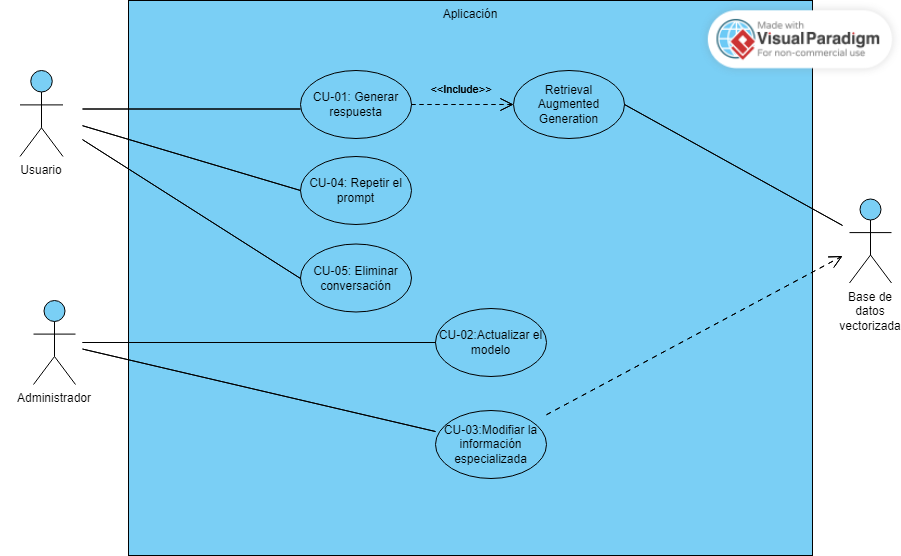
\includegraphics[width=1\textwidth]{img/usecase.png}
    \caption{Diagrama de casos de uso}
    \label{fig:usecase}
\end{figure}

En la figura \ref{fig:usecase} se puede ver un diagrama de casos de uso con tres actores principales, el usuario que es cualquier persona que utilice el programa para generar respuestas a sus cuestiones, el administrador que será el encargado del correcto funcionamiento del proyecto, gestionando los parámetros del modelo así cómo la información que dispone para el enriquecimiento y la base de datos vectorizada donde se almacenan los embeddings de la información con la que queramos enriquecer los prompts con el RAG.

\section{Explicación casos de uso.}

Se puede describir mediante el uso de tablas o mediante lenguaje natural.    

Una muestra de cómo podría ser una tabla de casos de uso:

% Caso de Uso 1 -> Consultar Experimentos.
\begin{table}[p]
	\centering
	\begin{tabularx}{\linewidth}{ p{0.21\columnwidth} p{0.71\columnwidth} }
		\toprule
		\textbf{CU-1}    & \textbf{Generar Respuesta}\\
		\toprule
		\textbf{Versión}              & 1.0    \\
		\textbf{Autor}                & Daniel de Lara Pérez \\
		\textbf{Requisitos asociados} & RF-1, RF-2, RF-3, RF-4, RF-5, RF-6 \\
		\textbf{Descripción}          & El usuario introduce, empleando lenguaje natural, una pregunta o solicitud al programa, esta pregunta se enriquecerá y un modelo generará una respuesta que se devuelve al usuario por pantalla \\
		\textbf{Precondición}         & El proyecto está iniciado \\
		\textbf{Acciones}             &
		\begin{enumerate}
			\def\labelenumi{\arabic{enumi}.}
			\tightlist
			\item El programa recibe la solicitud introducida por el usuario.
			\item Se vectoriza la solicitud para tener una representación matemática de la información.
   		\item El vector se compara, calculando su distancia, con los presentes en la base de datos vectorizada.
     	\item Se devuelve, junto con la solicitud inicial, la información cuya distancia al embedding de la solicitud sea más pequeña.
      	\item La solicitud inicial junto con el prompt son pasados al modelo para enriquecerlo y generar una respuesta especializada.
       	\item Se devuelve la respuesta al usuario.
        	\item El programa queda a la espera de una nueva solicitud.
         
		\end{enumerate}\\
		\textbf{Postcondición}        & La respuesta generada se devuelve al usuario. \\
		\textbf{Excepciones}          & Si el programa recibe una solicitud que no es capaz de procesar como caracteres especiales o lenguaje sin sentido se le informará al usuario \\
		\textbf{Importancia}          & Alta\\
		\bottomrule
	\end{tabularx}
	\caption{CU-1 Generar Respuesta.}
\end{table}

\begin{table}[p]
	\centering
	\begin{tabularx}{\linewidth}{ p{0.21\columnwidth} p{0.71\columnwidth} }
		\toprule
		\textbf{CU-2}    & \textbf{Actualizar el modelo}\\
		\toprule
		\textbf{Versión}              & 1.0    \\
		\textbf{Autor}                & Daniel de Lara Pérez \\
		\textbf{Requisitos asociados} & RF-10 \\
		\textbf{Descripción}          & El administrador modifica el código fuente afinando los valores que se le pasan al modelo como hiperparámetros \\
		\textbf{Precondición}         & El administrador tiene acceso al código fuente \\
		\textbf{Acciones}             &
		\begin{enumerate}
			\def\labelenumi{\arabic{enumi}.}
			\tightlist
			\item El administrador modifica los hiperparámetros por los que considere necesarios.
            \item Se vuelve a ejecutar el código fuente.
         
		\end{enumerate}\\
		\textbf{Postcondición}        & Futuras iteraciones del modelo generan respuestas con los nuevos hiperparámetros. \\
		\textbf{Excepciones}          &  \\
		\textbf{Importancia}          & Alta\\
		\bottomrule
	\end{tabularx}
	\caption{CU-2 Actualizar el modelo.}
\end{table}

\begin{table}[p]
	\centering
	\begin{tabularx}{\linewidth}{ p{0.21\columnwidth} p{0.71\columnwidth} }
		\toprule
		\textbf{CU-3}    & \textbf{Modificar la información especializada}\\
		\toprule
		\textbf{Versión}              & 1.0    \\
		\textbf{Autor}                & Daniel de Lara Pérez \\
		\textbf{Requisitos asociados} & RF-10 \\
		\textbf{Descripción}          & El administrador modifica la información contenida en la base de datos vectorizada, eliminando posibles datos erróneos, añadiendo nueva información o modificando el tema de la especialización. \\
		\textbf{Precondición}         & El administrador tiene acceso al archivo dónde se guarda la información \\
		\textbf{Acciones}             &
		\begin{enumerate}
			\def\labelenumi{\arabic{enumi}.}
			\tightlist
			\item El administrador modifica el archivo añadiendo o eliminando según considere para la tarea que se quiera realizar.
            \item Se vuelve a cargar el archivo con la información (Si el formato en el que se encuentra presentado cambia es posible que haya que modificar también el cargador)
            \item Se tokeniza la información si no se encuentra previamente en tokens establecidos.
            \item Se vuelve a ejecutar el código fuente.
         
		\end{enumerate}\\
		\textbf{Postcondición}        & Futuras iteraciones del modelo generan respuestas especialzadas con la nueva información. \\
		\textbf{Excepciones}          &  \\
		\textbf{Importancia}          & Alta\\
		\bottomrule
	\end{tabularx}
	\caption{CU-3 Modificar la información especializada.}
\end{table}

\begin{table}[p]
	\centering
	\begin{tabularx}{\linewidth}{ p{0.21\columnwidth} p{0.71\columnwidth} }
		\toprule
		\textbf{CU-4}    & \textbf{Repetir el prompt}\\
		\toprule
		\textbf{Versión}              & 1.0    \\
		\textbf{Autor}                & Daniel de Lara Pérez \\
		\textbf{Requisitos asociados} & RF-8 \\
		\textbf{Descripción}          & El usuario repite la misma pregunta para poder contrastar entre dos respuestas diferentes. \\
		\textbf{Precondición}         & El proyecto está iniciado y se ha generado una respuesta \\
		\textbf{Acciones}             &
		\begin{enumerate}
			\def\labelenumi{\arabic{enumi}.}
			\tightlist
			\item El usuario selecciona la opción de repetir el prompt
            \item El programa realiza la misma consulta ya realizada previamente
         
		\end{enumerate}\\
		\textbf{Postcondición}        & El usuario recibe una nueva consulta con el prompt previamente seleccionado. \\
		\textbf{Excepciones}          & No se ha introducido ningún prompt\\
		\textbf{Importancia}          & Media\\
		\bottomrule
	\end{tabularx}
	\caption{CU-4 Repetir el prompt.}
\end{table}

\begin{table}[p]
	\centering
	\begin{tabularx}{\linewidth}{ p{0.21\columnwidth} p{0.71\columnwidth} }
		\toprule
		\textbf{CU-5}    & \textbf{Eliminar conversación}\\
		\toprule
		\textbf{Versión}              & 1.0    \\
		\textbf{Autor}                & Daniel de Lara Pérez \\
		\textbf{Requisitos asociados} & RF-7 \\
		\textbf{Descripción}          & El usuario elimina la última interacción con el modelo o la conversación en su totalidad. \\
		\textbf{Precondición}         & El proyecto está iniciado y se ha generado, al menos, una respuesta \\
		\textbf{Acciones}             &
		\begin{enumerate}
			\def\labelenumi{\arabic{enumi}.}
			\tightlist
			\item El usuario selecciona la opción de eliminar última interacción o toda la conversación
            \item El programa elimina del registro la o las interacciones designadas
         
		\end{enumerate}\\
		\textbf{Postcondición}        & La o las consultas seleccionadas no se muestran por pantalla. \\
		\textbf{Excepciones}          &  No se ha introducido ningún prompt \\
		\textbf{Importancia}          & Baja\\
		\bottomrule
	\end{tabularx}
	\caption{CU-5 Eliminar conversación.}
\end{table}

\section{Prototipos de interfaz o interacción con el proyecto.}

Para este proyecto se ha desarrollado una interfaz de usuario básica que se puede ver en las imágenes \ref{fig:guivacia} y \ref{fig:guirellena}
\apendice{Estudio experimental}

En este apéndice se mostrarán y explicarán las distintas pruebas que se realizaron así cómo las condiciones en las que se realizaron y su discusión.

\section{Cuaderno de trabajo.}

Se enumeran todos los métodos probados con resultados positivos o no.

1.- Primero se intentó realizar el prpyecto en un entorno local mediante el editor de texto Visual Studio y un modelo pequeño de Mistral así cómo una versión preliminar de una aplicación Web empleando Streamlit, sin embargo los resultados que se obtuvieron con ese modelo eran bastante malos y no se parecían a las salidas esperadas.

2.- Tras el fracaso del primer modelo se probó a actualizar al Mistral 7B sin embargo, las librerías necesarias para ejecutarlo así cómo el tamaño del modelo hizo imposible la ejecución en local por lo que se pasó a los entornos virtuales, en este caso Google Colab que permite la aceleración de gpu de forma gratuita.

3.- Se cambió la interfaz gráfica de usuario de Streamlit ya que, el gran tamaño de la tecnología empleada hacía que fuera imposible lanzar la aplicación a la web sin emplear espacios de pago con gran GPU por lo que al final se decantó por emplear demos temporales en Gradio con posibilidad de mejora a entornos permanentes.

4.- En las primeras pruebas del modelo se usaron prompts sencillos y sin técnicas de prompt engineering y se obtenían resultados a veces buenos pero otras veces el lenguaje de la salida era confuso y con los espacios mal puestos un ejemplo:

Prompt: Specify the symptoms of covid-19

Salida: According to multiple scientific publications, including those retrieved through bibliographical searches in PubMed andGoogleScholar (as mentioned in two documents provided),thesymptomsofcovid-19canbebroadly categorisedintogeneralandorgan-specificmanifestations.ThemostcommonpersistsingsymptomsafterrecoveryfromtheinitialphaseofthesicknessexcludefatigueseveraltypesofrespiratorysymsptoonsuchascoughdyspniamuscleorpainjointpainguittylossofsensetasteormanosmiteshairlosssleepdifficultiesanxietydepressionSomeotherlessscommontypesofpost-CovidsignsalsoincludeskinrashthedescendedappeteatsweatinabilitytoconcentratememorylapseInadditiontothelsementsionedabove,somepatientshaveexperiencespecificorgandonsetcomplicationsmainlyaffectingtherespiratorsystemsuchaspulmonaledoafterhavingcontractedsarscov2whichmayresultinflammationpulmonaleumemonemodulationchronicobstructiveserialdisorderinterstitiallungdamagebronychiectasiapneumothoriastillheartkidneyneurosystemThesefindingsareconsistentwiththosereportedaSystematicReviewandaMeta-AnalyticoncludingthatfeversyllablemyalgianystiffinessheadacherecurrentnasalfissuresprickingorfierypathwayburningofthetonguepalatevaginaeyelashesdiarrheahighbloodedpressureshortstaturedizzyvisionblurredvisionspeechproblemmigrainesinsominolackoffeelingnumbesswellingsoftissuebruisingeczematouseruptionpurpletoenailspersistencethroughouthisstudydurationPatientswhopresenteditgastrointestinalsimptionslikeanorexicamalenourishmenthave ahigeriskfornegativeoutcomesItshouldbenotedhowevethatthemeta-analyticsmentionedearlierranksfevereccoughingfatiqueandsychronicallywerefoundtoprepresentthemeostprevalentsymbolsinpatientswithcovidduringtherefirstyearpandepticHowever,furthersubgroupsanalyzesbycontinenteitherconfirmedortrefutedslightvariationinfeprevrencefortheimentionedeightsymptonduetogeographicsfactorsTherefore,basedondifferentpublicationsreviewedthroughPubMediandoGooglesholarsearchdatabases,thefollowingsymptombscanbedassociatedwithcovid-19bothintheredynamicphasesandconvalescentperiodsafterwards:Febrewegghotfluidretainingaroundlegsfrequentlyunexplainedweightgainmuscleweaknessfataliguercoughbreathlessnesswheezingrapid breathinghigh temperaturelowgrade fevertirednessachinglimbsjoint swellingsleep disturbancesdigital clubbingchanges ingaitpatternanaemiahirsplittinghaemorraghsudden weight gainnew sensory perceptions like tinnitusrashing palpitatiopressure changesconstipationexcessive thirstdark urinecolicky abdominal discomfortpoornootritionreduced libidoextreme mood swingstrouble concentrateseeing spotsfloatersdouble visionlightheadednessdizzinessemesisprojectile vomitingwater bradozeophthalmosperiorbitaldiseasetremblingvoicechangeinyellowish eyesblack stoolsrectal bleedingerythmic irregularitycardiac arrhythmialiver cirrhosisstrokeparalyzing weaknessconvulsionelectrolyte imbalancedementiaAlthoughnotincludedinthenumberofdocumentsprovidedhere,itsworth notingthatlongtermeffectsoncognitivefuncdionhasalso beenidentifiedasa significant consequenceofcovid-19infectionespeciallyifleftuntreatedpromptlyReferencesavailable uponrequest

5.- Tras los malos resultados y, buscando la mejora en los resultados se emplearon técnicas de prompt engineering para comunicarse de manera eficiente con el modelo.

Prompt: Can you describe the symptoms of COVID-19, including both common and uncommon symptoms?

Salida: Based on several publications indexed in PubMed, the most frequent symptoms of COVID-19 are fever (up to 78\%), coughing (around 60\%), fatigue (approximately 33\%), and dyspnea (about 26\%) [1]. These findings come from a systematic review and meta-analysis covering over 132,000 infected individuals across multiple continents [1][2]. Common additional symptoms include but aren’t restricted to: 

Expectoration - mucous secretion when coughing; approximately 22\%.

Anosmia – loss of sense of smell; roughly 21\%, especially among those not previously diagnosed through traditional methods like temperature checks or CT scan results [1], although other sources suggest upwards of ~65\% depending upon population demographics [3].

Ageusia– lack of ability to perceive tastes; nearly half of affected persons report experiencing significant changes in flavor perception alongside olfactory issues [1].

Myalgias / Arthralgias – muscular \& bone pain respectively; affecting almost 17\%; often accompanied by weakness and stiffness [1].

Chills – shivers indicative of body cooling down involuntarily; present in close to 15\% of sufferers [1].

Headaches – occurring in just under 11\% of afflicted populations [1]; sometimes precede viral illness development [4].

Nausea or Vomiting – affects slightly above 8\% [1].

Rhinorrhea – runny nose; occurs within 8\% of subjects surveyed [1].

Hemoptsysi – bloodied sputum expelled via coughing; only seen in fewer than 3\% of respondents [1].

Longer term post-recovery impacts known colloquially as "long covid" consist of various lingering complaints lasting weeks to years past initial resolution of primary Covid-related symptoms. Such chronic problems span numerous organ systems—respiratory, cardiovascular, digestive, immunological, neuropsychologic etc., necessitating further research attention regarding diagnosis, prognosis, prevention strategies, treatments options, and overall impact assessment [2][3].

6.- Para mejorar aún más los resultados se realizaron técnicas de optimización de hiperparámetros lo que mejoró aún más los ya buenos resultados obtenidos.


\section{Configuración y parametrización de las técnicas.}

Para la generación del proyecto se empleo el modelo Mistral 7B con los siguientes hiperparámetros: 

\begin{itemize}

    \item Tarea: Generación de Texto
    \item Temperatura 0.2
    \item Penalización por repetición: %TODO
    \item Tokens máximos nuevos: 1000

\end{itemize}

Se seleccionó un valor bajo de la temperatura para que se ajuste a la información proporcionada y no genere datos inventados a partir de otra información que posea el modelo.

Para el entorno virtual en el que se realizaron las pruebas se seleccionó Google Colab con el Tipo de entorno de ejecución en Python 3 y el acelerador por hardware T4 GPU para ayudar a ejecutar las tareas costosas que ejecutará el modelo.

Para generar los prompts se emplearon las siguientes técnicas de prompt engineering:

\begin{itemize}
    \item \textbf{Claridad y Especificidad}: Los prompts están formulados de manera clara y específica para que el modelo entienda exactamente qué tipo de información se espera. Por ejemplo, se especifica que se deben incluir tanto síntomas comunes como menos comunes.
    \item \textbf{Contexto y Rol Asignado}: Al asignar un rol específico al modelo (por ejemplo, eres un experto en enfermedades infecciosas o eres un experto en salud pública), se le proporciona un contexto que le ayuda a generar una respuesta más informada y precisa.
    \item \textbf{Instrucciones Detalladas}: Se incluyen instrucciones detalladas para guiar la respuesta del modelo. Por ejemplo, se pide mencionar variaciones en los síntomas según la gravedad de la enfermedad o entre diferentes grupos de población.
    \item \textbf{Formato y Estructura}: La estructura del prompt está diseñada para ser lógica y coherente, comenzando con una petición clara y luego proporcionando detalles adicionales que deben ser incluidos.
    \item \textbf{Preguntas Abiertas y Específicas}: Se utilizan preguntas abiertas que permiten una respuesta detallada, pero también se asegura de que sean lo suficientemente específicas para evitar respuestas demasiado generales o fuera de tema.
\end{itemize}

\section{Detalle de resultados.}

Los resultados obtenidos en el proyecto son muchas veces los deseados, sin embargo en ocasiones hay que refinar el prompt por fallos en el modelo como por ejemplo, la pérdida de consistencia en los espacios de la salida aunque la información si que sea la correcta. Esto implica que para la obtención del resultado esperado se deban realizar varios intentos en algunos casos hasta obtener el mejor output posible. 
\apendice{Anexo de sostenibilización curricular}

\section{Introducción}
Este anexo incluirá una reflexión personal del alumnado sobre los aspectos de la sostenibilidad que se abordan en el trabajo.
Se pueden incluir tantas subsecciones como sean necesarias con la intención de explicar las competencias de sostenibilidad adquiridas durante el alumnado y aplicadas al Trabajo de Fin de Grado.

Más información en el documento de la CRUE \url{https://www.crue.org/wp-content/uploads/2020/02/Directrices_Sosteniblidad_Crue2012.pdf}.

Este anexo tendrá una extensión comprendida entre 600 y 800 palabras.



\bibliographystyle{apalike}
\bibliography{bibliografiaAnexos}

\end{document}
